\documentclass[12pt,landscape]{article}

%\usepackage{lmodern}
\usepackage{amssymb,amsmath}
\usepackage{bm}
\usepackage{graphicx}
\usepackage{microtype}
\usepackage{hyperref}
\pagestyle{empty}
\usepackage{titlesec}
\titleformat*{\section}{\LARGE\bfseries}
\titleformat*{\subsection}{\LARGE\bfseries}
\titleformat*{\subsubsection}{\LARGE\bfseries}
\setlength{\parindent}{0pt}
\setlength{\parskip}{1.2ex}
\setlength{\parindent}{0pt}
\setlength{\parskip}{1.2ex}

\setlength{\oddsidemargin}{-16mm}
\setlength{\textwidth}{260mm}
\setlength{\columnsep}{0.5in}
\setlength{\columnseprule}{1pt}
\setlength{\textheight}{202mm}
\setlength{\topmargin}{-32mm}
\setlength{\headsep}{0.25in}

\hypersetup
       {   pdfauthor = { Marco Fasondini },
           pdftitle={ foo },
           colorlinks=TRUE,
           linkcolor=black,
           citecolor=blue,
           urlcolor=blue
       }




\usepackage{upquote}
\usepackage{listings}
\usepackage{xcolor}
\lstset{
    basicstyle=\ttfamily\footnotesize,
    upquote=true,
    breaklines=true,
    breakindent=0pt,
    keepspaces=true,
    showspaces=false,
    columns=fullflexible,
    showtabs=false,
    showstringspaces=false,
    escapeinside={(*@}{@*)},
    extendedchars=true,
}
\newcommand{\HLJLt}[1]{#1}
\newcommand{\HLJLw}[1]{#1}
\newcommand{\HLJLe}[1]{#1}
\newcommand{\HLJLeB}[1]{#1}
\newcommand{\HLJLo}[1]{#1}
\newcommand{\HLJLk}[1]{\textcolor[RGB]{148,91,176}{\textbf{#1}}}
\newcommand{\HLJLkc}[1]{\textcolor[RGB]{59,151,46}{\textit{#1}}}
\newcommand{\HLJLkd}[1]{\textcolor[RGB]{214,102,97}{\textit{#1}}}
\newcommand{\HLJLkn}[1]{\textcolor[RGB]{148,91,176}{\textbf{#1}}}
\newcommand{\HLJLkp}[1]{\textcolor[RGB]{148,91,176}{\textbf{#1}}}
\newcommand{\HLJLkr}[1]{\textcolor[RGB]{148,91,176}{\textbf{#1}}}
\newcommand{\HLJLkt}[1]{\textcolor[RGB]{148,91,176}{\textbf{#1}}}
\newcommand{\HLJLn}[1]{#1}
\newcommand{\HLJLna}[1]{#1}
\newcommand{\HLJLnb}[1]{#1}
\newcommand{\HLJLnbp}[1]{#1}
\newcommand{\HLJLnc}[1]{#1}
\newcommand{\HLJLncB}[1]{#1}
\newcommand{\HLJLnd}[1]{\textcolor[RGB]{214,102,97}{#1}}
\newcommand{\HLJLne}[1]{#1}
\newcommand{\HLJLneB}[1]{#1}
\newcommand{\HLJLnf}[1]{\textcolor[RGB]{66,102,213}{#1}}
\newcommand{\HLJLnfm}[1]{\textcolor[RGB]{66,102,213}{#1}}
\newcommand{\HLJLnp}[1]{#1}
\newcommand{\HLJLnl}[1]{#1}
\newcommand{\HLJLnn}[1]{#1}
\newcommand{\HLJLno}[1]{#1}
\newcommand{\HLJLnt}[1]{#1}
\newcommand{\HLJLnv}[1]{#1}
\newcommand{\HLJLnvc}[1]{#1}
\newcommand{\HLJLnvg}[1]{#1}
\newcommand{\HLJLnvi}[1]{#1}
\newcommand{\HLJLnvm}[1]{#1}
\newcommand{\HLJLl}[1]{#1}
\newcommand{\HLJLld}[1]{\textcolor[RGB]{148,91,176}{\textit{#1}}}
\newcommand{\HLJLs}[1]{\textcolor[RGB]{201,61,57}{#1}}
\newcommand{\HLJLsa}[1]{\textcolor[RGB]{201,61,57}{#1}}
\newcommand{\HLJLsb}[1]{\textcolor[RGB]{201,61,57}{#1}}
\newcommand{\HLJLsc}[1]{\textcolor[RGB]{201,61,57}{#1}}
\newcommand{\HLJLsd}[1]{\textcolor[RGB]{201,61,57}{#1}}
\newcommand{\HLJLsdB}[1]{\textcolor[RGB]{201,61,57}{#1}}
\newcommand{\HLJLsdC}[1]{\textcolor[RGB]{201,61,57}{#1}}
\newcommand{\HLJLse}[1]{\textcolor[RGB]{59,151,46}{#1}}
\newcommand{\HLJLsh}[1]{\textcolor[RGB]{201,61,57}{#1}}
\newcommand{\HLJLsi}[1]{#1}
\newcommand{\HLJLso}[1]{\textcolor[RGB]{201,61,57}{#1}}
\newcommand{\HLJLsr}[1]{\textcolor[RGB]{201,61,57}{#1}}
\newcommand{\HLJLss}[1]{\textcolor[RGB]{201,61,57}{#1}}
\newcommand{\HLJLssB}[1]{\textcolor[RGB]{201,61,57}{#1}}
\newcommand{\HLJLnB}[1]{\textcolor[RGB]{59,151,46}{#1}}
\newcommand{\HLJLnbB}[1]{\textcolor[RGB]{59,151,46}{#1}}
\newcommand{\HLJLnfB}[1]{\textcolor[RGB]{59,151,46}{#1}}
\newcommand{\HLJLnh}[1]{\textcolor[RGB]{59,151,46}{#1}}
\newcommand{\HLJLni}[1]{\textcolor[RGB]{59,151,46}{#1}}
\newcommand{\HLJLnil}[1]{\textcolor[RGB]{59,151,46}{#1}}
\newcommand{\HLJLnoB}[1]{\textcolor[RGB]{59,151,46}{#1}}
\newcommand{\HLJLoB}[1]{\textcolor[RGB]{102,102,102}{\textbf{#1}}}
\newcommand{\HLJLow}[1]{\textcolor[RGB]{102,102,102}{\textbf{#1}}}
\newcommand{\HLJLp}[1]{#1}
\newcommand{\HLJLc}[1]{\textcolor[RGB]{153,153,119}{\textit{#1}}}
\newcommand{\HLJLch}[1]{\textcolor[RGB]{153,153,119}{\textit{#1}}}
\newcommand{\HLJLcm}[1]{\textcolor[RGB]{153,153,119}{\textit{#1}}}
\newcommand{\HLJLcp}[1]{\textcolor[RGB]{153,153,119}{\textit{#1}}}
\newcommand{\HLJLcpB}[1]{\textcolor[RGB]{153,153,119}{\textit{#1}}}
\newcommand{\HLJLcs}[1]{\textcolor[RGB]{153,153,119}{\textit{#1}}}
\newcommand{\HLJLcsB}[1]{\textcolor[RGB]{153,153,119}{\textit{#1}}}
\newcommand{\HLJLg}[1]{#1}
\newcommand{\HLJLgd}[1]{#1}
\newcommand{\HLJLge}[1]{#1}
\newcommand{\HLJLgeB}[1]{#1}
\newcommand{\HLJLgh}[1]{#1}
\newcommand{\HLJLgi}[1]{#1}
\newcommand{\HLJLgo}[1]{#1}
\newcommand{\HLJLgp}[1]{#1}
\newcommand{\HLJLgs}[1]{#1}
\newcommand{\HLJLgsB}[1]{#1}
\newcommand{\HLJLgt}[1]{#1}



\def\qqand{\qquad\hbox{and}\qquad}
\def\qqfor{\qquad\hbox{for}\qquad}
\def\qqas{\qquad\hbox{as}\qquad}
\def\half{ {1 \over 2} }
\def\D{ {\rm d} }
\def\I{ {\rm i} }
\def\E{ {\rm e} }
\def\C{ {\mathbb C} }
\def\R{ {\mathbb R} }
\def\H{ {\mathbb H} }
\def\Z{ {\mathbb Z} }
\def\CC{ {\cal C} }
\def\FF{ {\cal F} }
\def\HH{ {\cal H} }
\def\LL{ {\cal L} }
\def\vc#1{ {\mathbf #1} }
\def\bbC{ {\mathbb C} }



\def\fR{ f_{\rm R} }
\def\fL{ f_{\rm L} }

\def\qqqquad{\qquad\qquad}
\def\qqwhere{\qquad\hbox{where}\qquad}
\def\Res_#1{\underset{#1}{\rm Res}\,}
\def\sech{ {\rm sech}\, }
\def\acos{ {\rm acos}\, }
\def\asin{ {\rm asin}\, }
\def\atan{ {\rm atan}\, }
\def\Ei{ {\rm Ei}\, }
\def\upepsilon{\varepsilon}


\def\Xint#1{ \mathchoice
   {\XXint\displaystyle\textstyle{#1} }%
   {\XXint\textstyle\scriptstyle{#1} }%
   {\XXint\scriptstyle\scriptscriptstyle{#1} }%
   {\XXint\scriptscriptstyle\scriptscriptstyle{#1} }%
   \!\int}
\def\XXint#1#2#3{ {\setbox0=\hbox{$#1{#2#3}{\int}$}
     \vcenter{\hbox{$#2#3$}}\kern-.5\wd0} }
\def\ddashint{\Xint=}
\def\dashint{\Xint-}
% \def\dashint
\def\infdashint{\dashint_{-\infty}^\infty}




\def\addtab#1={#1\;&=}
\def\ccr{\\\addtab}
\def\ip<#1>{\left\langle{#1}\right\rangle}
\def\dx{\D x}
\def\dt{\D t}
\def\dz{\D z}
\def\ds{\D s}

\def\rR{ {\rm R} }
\def\rL{ {\rm L} }

\def\norm#1{\left\| #1 \right\|}

\def\pr(#1){\left({#1}\right)}
\def\br[#1]{\left[{#1}\right]}

\def\abs#1{\left|{#1}\right|}
\def\fpr(#1){\!\pr({#1})}

\def\sopmatrix#1{ \begin{pmatrix}#1\end{pmatrix} }

\def\endash{–}
\def\emdash{—}
\def\mdblksquare{\blacksquare}
\def\lgblksquare{\blacksquare}
\def\scre{\E}
\def\mapengine#1,#2.{\mapfunction{#1}\ifx\void#2\else\mapengine #2.\fi }

\def\map[#1]{\mapengine #1,\void.}

\def\mapenginesep_#1#2,#3.{\mapfunction{#2}\ifx\void#3\else#1\mapengine #3.\fi }

\def\mapsep_#1[#2]{\mapenginesep_{#1}#2,\void.}


\def\vcbr[#1]{\pr(#1)}


\def\bvect[#1,#2]{
{
\def\dots{\cdots}
\def\mapfunction##1{\ | \  ##1}
	\sopmatrix{
		 \,#1\map[#2]\,
	}
}
}



\def\vect[#1]{
{\def\dots{\ldots}
	\vcbr[{#1}]
} }

\def\vectt[#1]{
{\def\dots{\ldots}
	\vect[{#1}]^{\top}
} }

\def\Vectt[#1]{
{
\def\mapfunction##1{##1 \cr}
\def\dots{\vdots}
	\begin{pmatrix}
		\map[#1]
	\end{pmatrix}
} }

\def\addtab#1={#1\;&=}
\def\ccr{\\\addtab}

\def\questionequals{= \!\!\!\!\!\!{\scriptstyle ? \atop }\,\,\,}

\def\cent#1{\begin{center}#1\end{center} }

\lstset{
    basicstyle=\ttfamily,
	}

\begin{document}
{\LARGE
\sf
\textbf{Applied Complex Analysis (2021)}

\section{Lecture 19: Classical orthogonal polynomials}
We will also investigate the properties of \emph{classical} OPs. A good reference is  \href{http://dlmf.nist.gov/18}{Digital Library of Mathematical Functions, Chapter 18}.

This lecture we discuss

\begin{itemize}
\item[1. ] Hermite, Laguerre, and Jacobi polynomials


\item[2. ] Legendre, Chebyshev, and ultraspherical polynomials


\item[3. ] Explicit construction for Chebyshev polynomials

\end{itemize}
\subsection{Definition of classical orthogonal polynomials}
Classical orthogonal polynomials are orthogonal with respect to the following three weights:
\begin{center}
\begin{tabular}
{l | l | l | l | l}
Name & $(a,b)$ & $w(x)$ & Notation & $k_n$ \\
\hline
Hermite & $(-\infty,\infty)$ & $\E^{-x^2}$ & $H_n(x)$ & $2^n$ \\
Laguerre & $(0,\infty)$ & $x^\alpha \E^{-x}$ & $L_n^{(\alpha)}(x)$ & \href{http://dlmf.nist.gov/18.3}{Table 18.3.1} \\
Jacobi & $(-1,1)$ & $(1-x)^{\alpha} (1+x)^\beta$ & $P_n^{(\alpha,\beta)}(x)$ & \href{http://dlmf.nist.gov/18.3}{Table 18.3.1} \\
\end{tabular}
\end{center}
Note out of convention the parameters for Jacobi polynomials are right-to-left order.

We can actually construct these polynomials in Julia, first consider Hermite:


\begin{lstlisting}
(*@\HLJLk{using}@*) (*@\HLJLn{ApproxFun}@*)(*@\HLJLp{,}@*) (*@\HLJLn{Plots}@*)(*@\HLJLp{,}@*) (*@\HLJLn{LinearAlgebra}@*)(*@\HLJLp{,}@*) (*@\HLJLn{ComplexPhasePortrait}@*)
(*@\HLJLn{H\ensuremath{\_0}}@*) (*@\HLJLoB{=}@*) (*@\HLJLnf{Fun}@*)(*@\HLJLp{(}@*)(*@\HLJLnf{Hermite}@*)(*@\HLJLp{(),}@*) (*@\HLJLp{[}@*)(*@\HLJLni{1}@*)(*@\HLJLp{])}@*)
(*@\HLJLn{H\ensuremath{\_1}}@*) (*@\HLJLoB{=}@*) (*@\HLJLnf{Fun}@*)(*@\HLJLp{(}@*)(*@\HLJLnf{Hermite}@*)(*@\HLJLp{(),}@*) (*@\HLJLp{[}@*)(*@\HLJLni{0}@*)(*@\HLJLp{,}@*)(*@\HLJLni{1}@*)(*@\HLJLp{])}@*)
(*@\HLJLn{H\ensuremath{\_2}}@*) (*@\HLJLoB{=}@*) (*@\HLJLnf{Fun}@*)(*@\HLJLp{(}@*)(*@\HLJLnf{Hermite}@*)(*@\HLJLp{(),}@*) (*@\HLJLp{[}@*)(*@\HLJLni{0}@*)(*@\HLJLp{,}@*)(*@\HLJLni{0}@*)(*@\HLJLp{,}@*)(*@\HLJLni{1}@*)(*@\HLJLp{])}@*)
(*@\HLJLn{H\ensuremath{\_3}}@*) (*@\HLJLoB{=}@*) (*@\HLJLnf{Fun}@*)(*@\HLJLp{(}@*)(*@\HLJLnf{Hermite}@*)(*@\HLJLp{(),}@*) (*@\HLJLp{[}@*)(*@\HLJLni{0}@*)(*@\HLJLp{,}@*)(*@\HLJLni{0}@*)(*@\HLJLp{,}@*)(*@\HLJLni{0}@*)(*@\HLJLp{,}@*)(*@\HLJLni{1}@*)(*@\HLJLp{])}@*)
(*@\HLJLn{H\ensuremath{\_4}}@*) (*@\HLJLoB{=}@*) (*@\HLJLnf{Fun}@*)(*@\HLJLp{(}@*)(*@\HLJLnf{Hermite}@*)(*@\HLJLp{(),}@*) (*@\HLJLp{[}@*)(*@\HLJLni{0}@*)(*@\HLJLp{,}@*)(*@\HLJLni{0}@*)(*@\HLJLp{,}@*)(*@\HLJLni{0}@*)(*@\HLJLp{,}@*)(*@\HLJLni{0}@*)(*@\HLJLp{,}@*)(*@\HLJLni{1}@*)(*@\HLJLp{])}@*)
(*@\HLJLn{H\ensuremath{\_5}}@*) (*@\HLJLoB{=}@*) (*@\HLJLnf{Fun}@*)(*@\HLJLp{(}@*)(*@\HLJLnf{Hermite}@*)(*@\HLJLp{(),}@*) (*@\HLJLp{[}@*)(*@\HLJLni{0}@*)(*@\HLJLp{,}@*)(*@\HLJLni{0}@*)(*@\HLJLp{,}@*)(*@\HLJLni{0}@*)(*@\HLJLp{,}@*)(*@\HLJLni{0}@*)(*@\HLJLp{,}@*)(*@\HLJLni{0}@*)(*@\HLJLp{,}@*)(*@\HLJLni{1}@*)(*@\HLJLp{])}@*)

(*@\HLJLn{xx}@*) (*@\HLJLoB{=}@*) (*@\HLJLoB{-}@*)(*@\HLJLni{4}@*)(*@\HLJLoB{:}@*)(*@\HLJLnfB{0.01}@*)(*@\HLJLoB{:}@*)(*@\HLJLni{4}@*)
(*@\HLJLnf{plot}@*)(*@\HLJLp{(}@*)(*@\HLJLn{xx}@*)(*@\HLJLp{,}@*) (*@\HLJLn{H\ensuremath{\_0}}@*)(*@\HLJLoB{.}@*)(*@\HLJLp{(}@*)(*@\HLJLn{xx}@*)(*@\HLJLp{);}@*) (*@\HLJLn{label}@*)(*@\HLJLoB{=}@*)(*@\HLJLs{"{}H{\_}0"{}}@*)(*@\HLJLp{,}@*) (*@\HLJLn{ylims}@*)(*@\HLJLoB{=}@*)(*@\HLJLp{(}@*)(*@\HLJLoB{-}@*)(*@\HLJLni{400}@*)(*@\HLJLp{,}@*)(*@\HLJLni{400}@*)(*@\HLJLp{))}@*)
(*@\HLJLnf{plot!}@*)(*@\HLJLp{(}@*)(*@\HLJLn{xx}@*)(*@\HLJLp{,}@*) (*@\HLJLn{H\ensuremath{\_1}}@*)(*@\HLJLoB{.}@*)(*@\HLJLp{(}@*)(*@\HLJLn{xx}@*)(*@\HLJLp{);}@*) (*@\HLJLn{label}@*)(*@\HLJLoB{=}@*)(*@\HLJLs{"{}H{\_}1"{}}@*)(*@\HLJLp{,}@*) (*@\HLJLn{ylims}@*)(*@\HLJLoB{=}@*)(*@\HLJLp{(}@*)(*@\HLJLoB{-}@*)(*@\HLJLni{400}@*)(*@\HLJLp{,}@*)(*@\HLJLni{400}@*)(*@\HLJLp{))}@*)
(*@\HLJLnf{plot!}@*)(*@\HLJLp{(}@*)(*@\HLJLn{xx}@*)(*@\HLJLp{,}@*) (*@\HLJLn{H\ensuremath{\_2}}@*)(*@\HLJLoB{.}@*)(*@\HLJLp{(}@*)(*@\HLJLn{xx}@*)(*@\HLJLp{);}@*) (*@\HLJLn{label}@*)(*@\HLJLoB{=}@*)(*@\HLJLs{"{}H{\_}2"{}}@*)(*@\HLJLp{,}@*) (*@\HLJLn{ylims}@*)(*@\HLJLoB{=}@*)(*@\HLJLp{(}@*)(*@\HLJLoB{-}@*)(*@\HLJLni{400}@*)(*@\HLJLp{,}@*)(*@\HLJLni{400}@*)(*@\HLJLp{))}@*)
(*@\HLJLnf{plot!}@*)(*@\HLJLp{(}@*)(*@\HLJLn{xx}@*)(*@\HLJLp{,}@*) (*@\HLJLn{H\ensuremath{\_3}}@*)(*@\HLJLoB{.}@*)(*@\HLJLp{(}@*)(*@\HLJLn{xx}@*)(*@\HLJLp{);}@*) (*@\HLJLn{label}@*)(*@\HLJLoB{=}@*)(*@\HLJLs{"{}H{\_}3"{}}@*)(*@\HLJLp{,}@*) (*@\HLJLn{ylims}@*)(*@\HLJLoB{=}@*)(*@\HLJLp{(}@*)(*@\HLJLoB{-}@*)(*@\HLJLni{400}@*)(*@\HLJLp{,}@*)(*@\HLJLni{400}@*)(*@\HLJLp{))}@*)
(*@\HLJLnf{plot!}@*)(*@\HLJLp{(}@*)(*@\HLJLn{xx}@*)(*@\HLJLp{,}@*) (*@\HLJLn{H\ensuremath{\_4}}@*)(*@\HLJLoB{.}@*)(*@\HLJLp{(}@*)(*@\HLJLn{xx}@*)(*@\HLJLp{);}@*) (*@\HLJLn{label}@*)(*@\HLJLoB{=}@*)(*@\HLJLs{"{}H{\_}4"{}}@*)(*@\HLJLp{,}@*) (*@\HLJLn{ylims}@*)(*@\HLJLoB{=}@*)(*@\HLJLp{(}@*)(*@\HLJLoB{-}@*)(*@\HLJLni{400}@*)(*@\HLJLp{,}@*)(*@\HLJLni{400}@*)(*@\HLJLp{))}@*)
(*@\HLJLnf{plot!}@*)(*@\HLJLp{(}@*)(*@\HLJLn{xx}@*)(*@\HLJLp{,}@*) (*@\HLJLn{H\ensuremath{\_5}}@*)(*@\HLJLoB{.}@*)(*@\HLJLp{(}@*)(*@\HLJLn{xx}@*)(*@\HLJLp{);}@*) (*@\HLJLn{label}@*)(*@\HLJLoB{=}@*)(*@\HLJLs{"{}H{\_}5"{}}@*)(*@\HLJLp{)}@*)
\end{lstlisting}

\cent{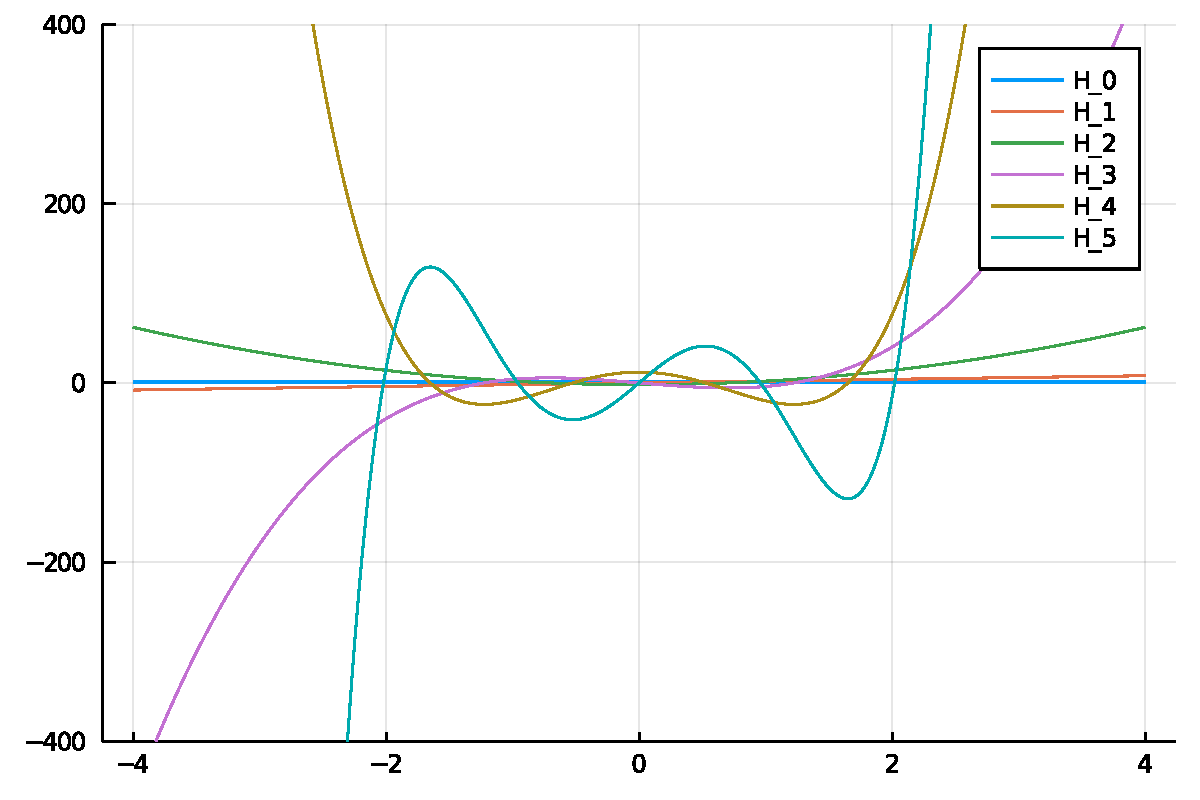
\includegraphics[width=0.75\linewidth]{C:/Users/mfaso/OneDrive/Documents/GitHub/M3M6AppliedComplexAnalysis/output/figures/Lecture19_1_1.pdf}}

We verify their orthogonality:


\begin{lstlisting}
(*@\HLJLn{w}@*) (*@\HLJLoB{=}@*) (*@\HLJLnf{Fun}@*)(*@\HLJLp{(}@*)(*@\HLJLnf{GaussWeight}@*)(*@\HLJLp{(),}@*) (*@\HLJLp{[}@*)(*@\HLJLnfB{1.0}@*)(*@\HLJLp{])}@*)

(*@\HLJLnd{@show}@*) (*@\HLJLnf{sum}@*)(*@\HLJLp{(}@*)(*@\HLJLn{H\ensuremath{\_2}}@*)(*@\HLJLoB{*}@*)(*@\HLJLn{H\ensuremath{\_5}}@*)(*@\HLJLoB{*}@*)(*@\HLJLn{w}@*)(*@\HLJLp{)}@*)  (*@\HLJLcs{{\#}}@*) (*@\HLJLcs{means}@*) (*@\HLJLcs{integrate}@*)
(*@\HLJLnd{@show}@*) (*@\HLJLnf{sum}@*)(*@\HLJLp{(}@*)(*@\HLJLn{H\ensuremath{\_5}}@*)(*@\HLJLoB{*}@*)(*@\HLJLn{H\ensuremath{\_5}}@*)(*@\HLJLoB{*}@*)(*@\HLJLn{w}@*)(*@\HLJLp{);}@*)
\end{lstlisting}

\begin{lstlisting}
sum(H_2 * H_5 * w) = 0.0  
sum(H_5 * H_5 * w) = 6806.222787477181
\end{lstlisting}


Now Jacobi:


\begin{lstlisting}
(*@\HLJLn{\ensuremath{\alpha}}@*)(*@\HLJLp{,}@*)(*@\HLJLn{\ensuremath{\beta}}@*) (*@\HLJLoB{=}@*) (*@\HLJLnfB{0.1}@*)(*@\HLJLp{,}@*)(*@\HLJLnfB{0.2}@*)
(*@\HLJLn{P\ensuremath{\_0}}@*) (*@\HLJLoB{=}@*) (*@\HLJLnf{Fun}@*)(*@\HLJLp{(}@*)(*@\HLJLnf{Jacobi}@*)(*@\HLJLp{(}@*)(*@\HLJLn{\ensuremath{\beta}}@*)(*@\HLJLp{,}@*)(*@\HLJLn{\ensuremath{\alpha}}@*)(*@\HLJLp{),}@*) (*@\HLJLp{[}@*)(*@\HLJLni{1}@*)(*@\HLJLp{])}@*)
(*@\HLJLn{P\ensuremath{\_1}}@*) (*@\HLJLoB{=}@*) (*@\HLJLnf{Fun}@*)(*@\HLJLp{(}@*)(*@\HLJLnf{Jacobi}@*)(*@\HLJLp{(}@*)(*@\HLJLn{\ensuremath{\beta}}@*)(*@\HLJLp{,}@*)(*@\HLJLn{\ensuremath{\alpha}}@*)(*@\HLJLp{),}@*) (*@\HLJLp{[}@*)(*@\HLJLni{0}@*)(*@\HLJLp{,}@*)(*@\HLJLni{1}@*)(*@\HLJLp{])}@*)
(*@\HLJLn{P\ensuremath{\_2}}@*) (*@\HLJLoB{=}@*) (*@\HLJLnf{Fun}@*)(*@\HLJLp{(}@*)(*@\HLJLnf{Jacobi}@*)(*@\HLJLp{(}@*)(*@\HLJLn{\ensuremath{\beta}}@*)(*@\HLJLp{,}@*)(*@\HLJLn{\ensuremath{\alpha}}@*)(*@\HLJLp{),}@*) (*@\HLJLp{[}@*)(*@\HLJLni{0}@*)(*@\HLJLp{,}@*)(*@\HLJLni{0}@*)(*@\HLJLp{,}@*)(*@\HLJLni{1}@*)(*@\HLJLp{])}@*)
(*@\HLJLn{P\ensuremath{\_3}}@*) (*@\HLJLoB{=}@*) (*@\HLJLnf{Fun}@*)(*@\HLJLp{(}@*)(*@\HLJLnf{Jacobi}@*)(*@\HLJLp{(}@*)(*@\HLJLn{\ensuremath{\beta}}@*)(*@\HLJLp{,}@*)(*@\HLJLn{\ensuremath{\alpha}}@*)(*@\HLJLp{),}@*) (*@\HLJLp{[}@*)(*@\HLJLni{0}@*)(*@\HLJLp{,}@*)(*@\HLJLni{0}@*)(*@\HLJLp{,}@*)(*@\HLJLni{0}@*)(*@\HLJLp{,}@*)(*@\HLJLni{1}@*)(*@\HLJLp{])}@*)
(*@\HLJLn{P\ensuremath{\_4}}@*) (*@\HLJLoB{=}@*) (*@\HLJLnf{Fun}@*)(*@\HLJLp{(}@*)(*@\HLJLnf{Jacobi}@*)(*@\HLJLp{(}@*)(*@\HLJLn{\ensuremath{\beta}}@*)(*@\HLJLp{,}@*)(*@\HLJLn{\ensuremath{\alpha}}@*)(*@\HLJLp{),}@*) (*@\HLJLp{[}@*)(*@\HLJLni{0}@*)(*@\HLJLp{,}@*)(*@\HLJLni{0}@*)(*@\HLJLp{,}@*)(*@\HLJLni{0}@*)(*@\HLJLp{,}@*)(*@\HLJLni{0}@*)(*@\HLJLp{,}@*)(*@\HLJLni{1}@*)(*@\HLJLp{])}@*)
(*@\HLJLn{P\ensuremath{\_5}}@*) (*@\HLJLoB{=}@*) (*@\HLJLnf{Fun}@*)(*@\HLJLp{(}@*)(*@\HLJLnf{Jacobi}@*)(*@\HLJLp{(}@*)(*@\HLJLn{\ensuremath{\beta}}@*)(*@\HLJLp{,}@*)(*@\HLJLn{\ensuremath{\alpha}}@*)(*@\HLJLp{),}@*) (*@\HLJLp{[}@*)(*@\HLJLni{0}@*)(*@\HLJLp{,}@*)(*@\HLJLni{0}@*)(*@\HLJLp{,}@*)(*@\HLJLni{0}@*)(*@\HLJLp{,}@*)(*@\HLJLni{0}@*)(*@\HLJLp{,}@*)(*@\HLJLni{0}@*)(*@\HLJLp{,}@*)(*@\HLJLni{1}@*)(*@\HLJLp{])}@*)

(*@\HLJLn{xx}@*) (*@\HLJLoB{=}@*) (*@\HLJLoB{-}@*)(*@\HLJLni{1}@*)(*@\HLJLoB{:}@*)(*@\HLJLnfB{0.01}@*)(*@\HLJLoB{:}@*)(*@\HLJLni{1}@*)
(*@\HLJLnf{plot}@*)(*@\HLJLp{(}@*) (*@\HLJLn{xx}@*)(*@\HLJLp{,}@*) (*@\HLJLn{P\ensuremath{\_0}}@*)(*@\HLJLoB{.}@*)(*@\HLJLp{(}@*)(*@\HLJLn{xx}@*)(*@\HLJLp{);}@*) (*@\HLJLn{label}@*)(*@\HLJLoB{=}@*)(*@\HLJLs{"{}P{\_}0{\textasciicircum}(}@*)(*@\HLJLsi{{\$}\ensuremath{\alpha}}@*)(*@\HLJLs{,}@*)(*@\HLJLsi{{\$}\ensuremath{\beta}}@*)(*@\HLJLs{)"{}}@*)(*@\HLJLp{,}@*) (*@\HLJLn{ylims}@*)(*@\HLJLoB{=}@*)(*@\HLJLp{(}@*)(*@\HLJLoB{-}@*)(*@\HLJLni{2}@*)(*@\HLJLp{,}@*)(*@\HLJLni{2}@*)(*@\HLJLp{))}@*)
(*@\HLJLnf{plot!}@*)(*@\HLJLp{(}@*)(*@\HLJLn{xx}@*)(*@\HLJLp{,}@*) (*@\HLJLn{P\ensuremath{\_1}}@*)(*@\HLJLoB{.}@*)(*@\HLJLp{(}@*)(*@\HLJLn{xx}@*)(*@\HLJLp{);}@*) (*@\HLJLn{label}@*)(*@\HLJLoB{=}@*)(*@\HLJLs{"{}P{\_}1{\textasciicircum}(}@*)(*@\HLJLsi{{\$}\ensuremath{\alpha}}@*)(*@\HLJLs{,}@*)(*@\HLJLsi{{\$}\ensuremath{\beta}}@*)(*@\HLJLs{)"{}}@*)(*@\HLJLp{)}@*)
(*@\HLJLnf{plot!}@*)(*@\HLJLp{(}@*)(*@\HLJLn{xx}@*)(*@\HLJLp{,}@*) (*@\HLJLn{P\ensuremath{\_2}}@*)(*@\HLJLoB{.}@*)(*@\HLJLp{(}@*)(*@\HLJLn{xx}@*)(*@\HLJLp{);}@*) (*@\HLJLn{label}@*)(*@\HLJLoB{=}@*)(*@\HLJLs{"{}P{\_}2{\textasciicircum}(}@*)(*@\HLJLsi{{\$}\ensuremath{\alpha}}@*)(*@\HLJLs{,}@*)(*@\HLJLsi{{\$}\ensuremath{\beta}}@*)(*@\HLJLs{)"{}}@*)(*@\HLJLp{)}@*)
(*@\HLJLnf{plot!}@*)(*@\HLJLp{(}@*)(*@\HLJLn{xx}@*)(*@\HLJLp{,}@*) (*@\HLJLn{P\ensuremath{\_3}}@*)(*@\HLJLoB{.}@*)(*@\HLJLp{(}@*)(*@\HLJLn{xx}@*)(*@\HLJLp{);}@*) (*@\HLJLn{label}@*)(*@\HLJLoB{=}@*)(*@\HLJLs{"{}P{\_}3{\textasciicircum}(}@*)(*@\HLJLsi{{\$}\ensuremath{\alpha}}@*)(*@\HLJLs{,}@*)(*@\HLJLsi{{\$}\ensuremath{\beta}}@*)(*@\HLJLs{)"{}}@*)(*@\HLJLp{)}@*)
(*@\HLJLnf{plot!}@*)(*@\HLJLp{(}@*)(*@\HLJLn{xx}@*)(*@\HLJLp{,}@*) (*@\HLJLn{P\ensuremath{\_4}}@*)(*@\HLJLoB{.}@*)(*@\HLJLp{(}@*)(*@\HLJLn{xx}@*)(*@\HLJLp{);}@*) (*@\HLJLn{label}@*)(*@\HLJLoB{=}@*)(*@\HLJLs{"{}P{\_}4{\textasciicircum}(}@*)(*@\HLJLsi{{\$}\ensuremath{\alpha}}@*)(*@\HLJLs{,}@*)(*@\HLJLsi{{\$}\ensuremath{\beta}}@*)(*@\HLJLs{)"{}}@*)(*@\HLJLp{)}@*)
(*@\HLJLnf{plot!}@*)(*@\HLJLp{(}@*)(*@\HLJLn{xx}@*)(*@\HLJLp{,}@*) (*@\HLJLn{P\ensuremath{\_5}}@*)(*@\HLJLoB{.}@*)(*@\HLJLp{(}@*)(*@\HLJLn{xx}@*)(*@\HLJLp{);}@*) (*@\HLJLn{label}@*)(*@\HLJLoB{=}@*)(*@\HLJLs{"{}P{\_}5{\textasciicircum}(}@*)(*@\HLJLsi{{\$}\ensuremath{\alpha}}@*)(*@\HLJLs{,}@*)(*@\HLJLsi{{\$}\ensuremath{\beta}}@*)(*@\HLJLs{)"{}}@*)(*@\HLJLp{)}@*)
\end{lstlisting}

\cent{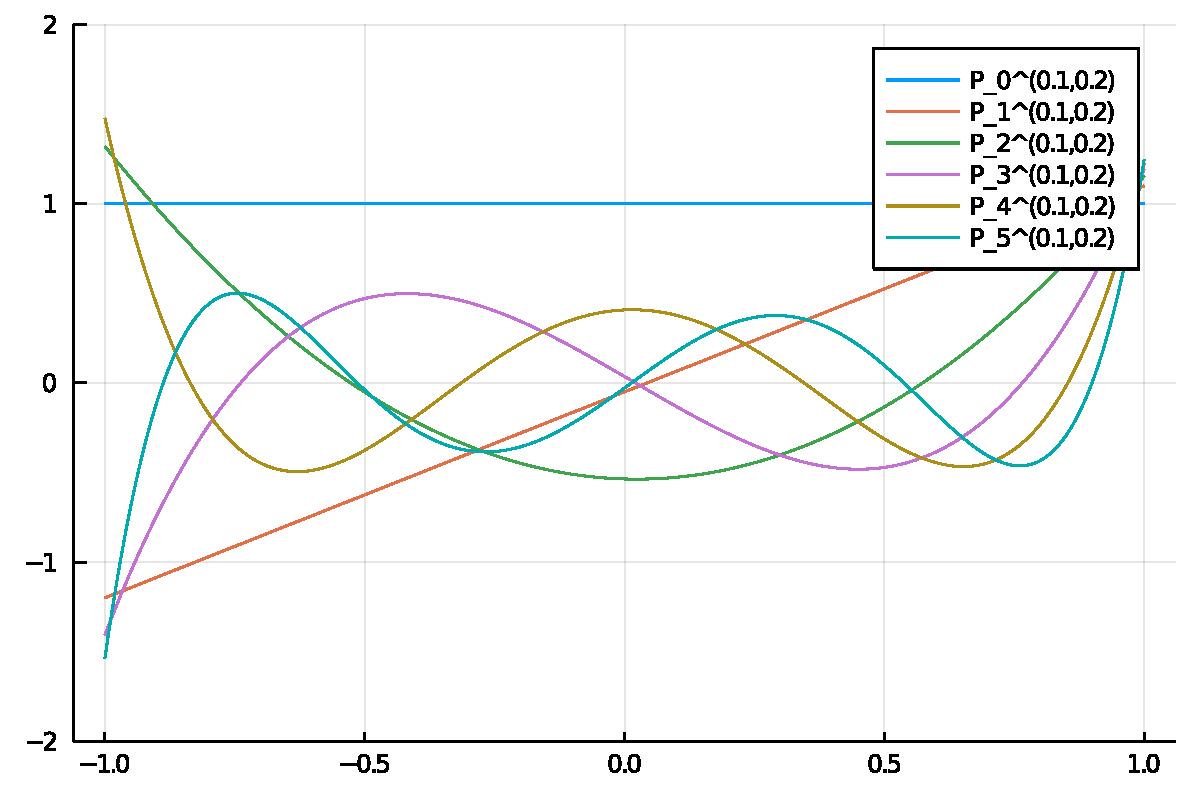
\includegraphics[width=0.85\linewidth]{C:/Users/mfaso/OneDrive/Documents/GitHub/M3M6AppliedComplexAnalysis/output/figures/Lecture19_3_1.pdf}}

\begin{lstlisting}
(*@\HLJLn{w}@*) (*@\HLJLoB{=}@*) (*@\HLJLnf{Fun}@*)(*@\HLJLp{(}@*)(*@\HLJLnf{JacobiWeight}@*)(*@\HLJLp{(}@*)(*@\HLJLn{\ensuremath{\beta}}@*)(*@\HLJLp{,}@*)(*@\HLJLn{\ensuremath{\alpha}}@*)(*@\HLJLp{),}@*) (*@\HLJLp{[}@*)(*@\HLJLnfB{1.0}@*)(*@\HLJLp{])}@*)
(*@\HLJLnd{@show}@*) (*@\HLJLnf{sum}@*)(*@\HLJLp{(}@*)(*@\HLJLn{P\ensuremath{\_2}}@*)(*@\HLJLoB{*}@*)(*@\HLJLn{P\ensuremath{\_5}}@*)(*@\HLJLoB{*}@*)(*@\HLJLn{w}@*)(*@\HLJLp{)}@*)  (*@\HLJLcs{{\#}}@*) (*@\HLJLcs{means}@*) (*@\HLJLcs{integrate}@*)
(*@\HLJLnd{@show}@*) (*@\HLJLnf{sum}@*)(*@\HLJLp{(}@*)(*@\HLJLn{P\ensuremath{\_5}}@*)(*@\HLJLoB{*}@*)(*@\HLJLn{P\ensuremath{\_5}}@*)(*@\HLJLoB{*}@*)(*@\HLJLn{w}@*)(*@\HLJLp{);}@*)
\end{lstlisting}

\begin{lstlisting}
sum(P(*@\ensuremath{\_2} * P{\_5} * w) = -1.235990476633475e-17\\
sum(P{\_5} * P{\_5} * w) = 0.21713358248393155
\end{lstlisting}


\subsection{Legendre, Chebyshev, and ultraspherical polynomials}
There are special families of Jacobi weights with their own name.

\begin{tabular}
{l | l | l | l | l}
Name & Jacobi parameters & $w(x)$ & Notation & $k_n$ \\
\hline
Jacobi & $\alpha,\beta$ & $(1-x)^{\alpha} (1+x)^\beta$ & $P_n^{(\alpha,\beta)}(x)$ & \href{http://dlmf.nist.gov/18.3}{Table 18.3.1} \\
Legendre & $0,0$ & $1$ & $P_n(x)$ & $2^n(1/2)_n/n!$ \\
Chebyshev (1st) & $-{1 \over 2},-{1 \over 2}$ & $1 \over \sqrt{1-x^2}$ & $T_n(x)$ & $1 (n=0), 2^{n-1} (n \neq 0)$ \\
Chebyshev (2nd) & ${1 \over 2},{1 \over 2}$ & $\sqrt{1-x^2}$ & $U_n(x)$ & $2^n$ \\
Ultraspherical & $\lambda-{1 \over 2},\lambda-{1 \over 2}$ & $(1-x^2)^{\lambda - 1/2}, \lambda \neq 0$ & $C_n^{(\lambda)}(x)$ & $2^n(\lambda)_n/n!$ \\
\end{tabular}
Note that other than Legendre, these polynomials have a different normalization than $P_n^{(\alpha,\beta)}$:


\begin{lstlisting}
(*@\HLJLn{T\ensuremath{\_2}}@*) (*@\HLJLoB{=}@*) (*@\HLJLnf{Fun}@*)(*@\HLJLp{(}@*)(*@\HLJLnf{Chebyshev}@*)(*@\HLJLp{(),}@*) (*@\HLJLp{[}@*)(*@\HLJLnfB{0.0}@*)(*@\HLJLp{,}@*)(*@\HLJLni{0}@*)(*@\HLJLp{,}@*)(*@\HLJLni{1}@*)(*@\HLJLp{])}@*)
(*@\HLJLn{P\ensuremath{\_2}}@*) (*@\HLJLoB{=}@*) (*@\HLJLnf{Fun}@*)(*@\HLJLp{(}@*)(*@\HLJLnf{Jacobi}@*)(*@\HLJLp{(}@*)(*@\HLJLoB{-}@*)(*@\HLJLni{1}@*)(*@\HLJLoB{/}@*)(*@\HLJLni{2}@*)(*@\HLJLp{,}@*)(*@\HLJLoB{-}@*)(*@\HLJLni{1}@*)(*@\HLJLoB{/}@*)(*@\HLJLni{2}@*)(*@\HLJLp{),}@*) (*@\HLJLp{[}@*)(*@\HLJLnfB{0.0}@*)(*@\HLJLp{,}@*)(*@\HLJLni{0}@*)(*@\HLJLp{,}@*)(*@\HLJLni{1}@*)(*@\HLJLp{])}@*)
(*@\HLJLnf{plot}@*)(*@\HLJLp{(}@*)(*@\HLJLn{T\ensuremath{\_2}}@*)(*@\HLJLp{;}@*) (*@\HLJLn{label}@*)(*@\HLJLoB{=}@*)(*@\HLJLs{"{}T{\_}2"{}}@*)(*@\HLJLp{,}@*) (*@\HLJLn{title}@*)(*@\HLJLoB{=}@*)(*@\HLJLs{"{}T{\_}2}@*) (*@\HLJLs{is}@*) (*@\HLJLs{C*P{\_}2}@*) (*@\HLJLs{for}@*) (*@\HLJLs{some}@*) (*@\HLJLs{C"{}}@*)(*@\HLJLp{)}@*)
(*@\HLJLnf{plot!}@*)(*@\HLJLp{(}@*)(*@\HLJLn{P\ensuremath{\_2}}@*)(*@\HLJLp{;}@*) (*@\HLJLn{label}@*)(*@\HLJLoB{=}@*)(*@\HLJLs{"{}P{\_}2"{}}@*)(*@\HLJLp{)}@*)
\end{lstlisting}

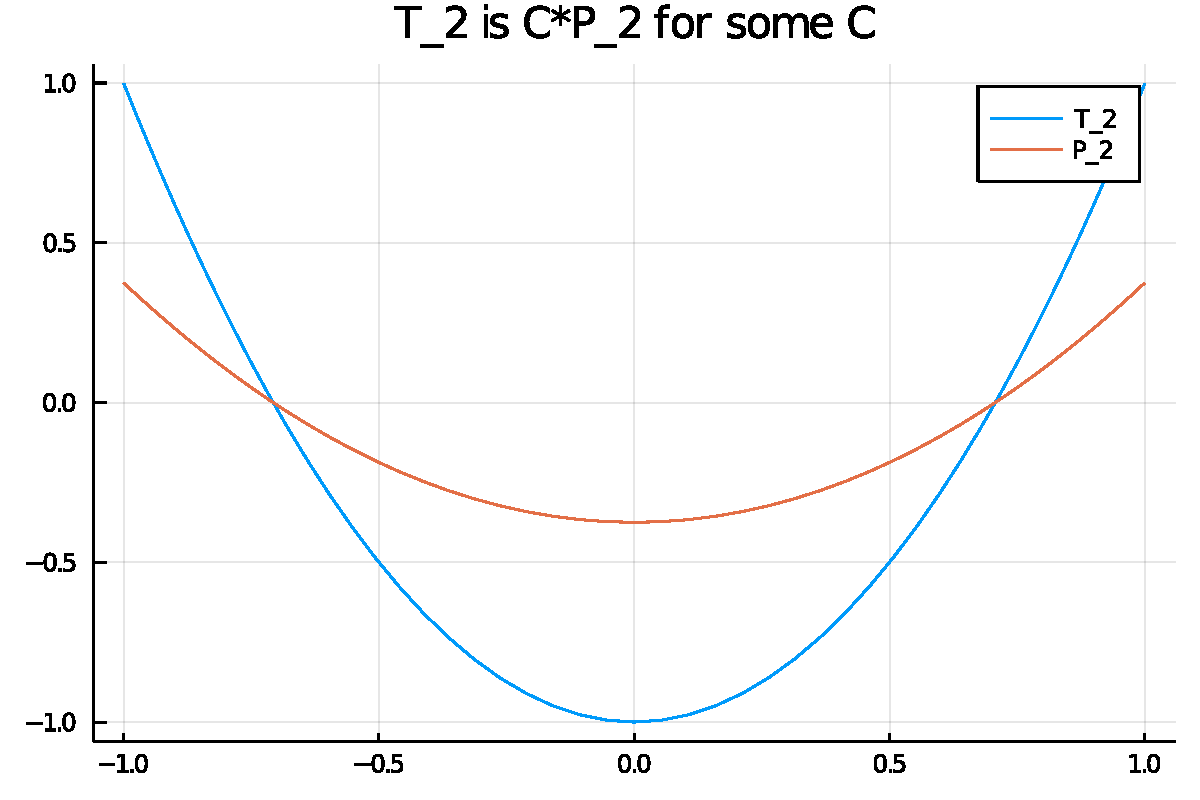
\includegraphics[width=\linewidth]{C:/Users/mfaso/OneDrive/Documents/GitHub/M3M6AppliedComplexAnalysis/output/figures/Lecture19_5_1.pdf}

But because they are orthogonal w.r.t. the same weight, they must be a constant multiple of each-other, as discussed last lecture.

\subsubsection{Explicit construction of Chebyshev polynomials (first kind and second kind)}
Chebyshev polynomials are pretty much the only OPs with \emph{simple} closed form expressions.

\textbf{Proposition (Chebyshev first kind formula)} $T_n(x) = \cos n \acos x$ or in other words,

\[
T_n(\cos \theta) = \cos n \theta
\]
\textbf{Proof} We first show that they are orthogonal w.r.t. $1/\sqrt{1-x^2}$. Too easy: do $x = \cos \theta$, $\dx = -\sin \theta$ to get (for $n \neq m$)


\begin{align*}
    \int_{-1}^1 {\cos n \acos x \cos m \acos x \dx \over \sqrt{1-x^2}} &= -\int_\pi^0  \cos n \theta \cos m \theta \D \theta \ccr
    =  \int_0^\pi  {\E^{\I (-n-m)\theta} + \E^{\I (n-m)\theta} + \E^{\I (m-n)\theta} + \E^{\I (n+m)\theta}    \over 4} \D \theta =0
\end{align*}
\newpage
We then need to show it has the right highest order term $k_n$. Note that $k_0 = k_1 = 1$.  Using $z = \E^{\I \theta}$ we see that $\cos n \theta$ has a simple recurrence for $n=2,3,\ldots$:

\[
\cos n \theta = {z^n + z^{-n} \over 2} = 2 {z + z^{-1} \over 2} {z^{n-1} + z^{1-n} \over 2}- {z^{n-2} + z^{2-n} \over 2} =
2 \cos \theta \cos (n-1)\theta - \cos(n-2)\theta
\]
thus

\[
\cos n \acos x = 2 x \cos(n-1) \acos x - \cos(n-2) \acos x
\]
It follows that

\[
k_n = 2 k_{n-1} = 2^{n-1} k_1 = 2^{n-1}
\]
By uniqueness we have $T_n(x) = \cos n \acos x$.

\ensuremath{\blacksquare}
\
\textbf{Proposition (Chebyshev second kind formula)} $U_n(x) = {\sin (n+1) \acos x \over \sin \acos x}$ or in other words,

\[
U_n(\cos \theta) = {\sin (n+1) \theta \over \sin \theta}
\]
\newpage
\emph{Example} For the case of Chebyshev polynomials, we have

\[
J = \begin{pmatrix}
0 & 1 \cr
\half & 0 & \half \cr
& \half & 0 & \half \cr
&& \half & 0 & \ddots \cr
&&&\ddots & \ddots
\end{pmatrix}
\]
Therefore, the Chebyshev coefficients of $x f(x)$ are given by

\[
J^\top \vc f = \begin{pmatrix}
0 & \half \cr
1 & 0 & \half \cr
& \half & 0 & \half \cr
&& \half & 0 & \ddots \cr
&&&\ddots & \ddots
\end{pmatrix} \begin{pmatrix} f_0\\ f_1\\f_2\\f_3\\\vdots\end{pmatrix}
\]
\subsubsection{Demonstration}
In the case where $f$ is a degree $n-1$  polynomial, we can represent $J^\top$ as an $n+1 \times n$ matrix (this makes sense as $x f(x)$ is one more degree than $f$):


\begin{lstlisting}
(*@\HLJLn{f}@*) (*@\HLJLoB{=}@*) (*@\HLJLnf{Fun}@*)(*@\HLJLp{(}@*)(*@\HLJLn{exp}@*)(*@\HLJLp{,}@*) (*@\HLJLnf{Chebyshev}@*)(*@\HLJLp{())}@*)
(*@\HLJLn{n}@*) (*@\HLJLoB{=}@*) (*@\HLJLnf{ncoefficients}@*)(*@\HLJLp{(}@*)(*@\HLJLn{f}@*)(*@\HLJLp{)}@*) (*@\HLJLcs{{\#}}@*) (*@\HLJLcs{number}@*) (*@\HLJLcs{of}@*) (*@\HLJLcs{coefficients}@*)
(*@\HLJLnd{@show}@*) (*@\HLJLn{n}@*)
(*@\HLJLn{J}@*) (*@\HLJLoB{=}@*) (*@\HLJLnf{zeros}@*)(*@\HLJLp{(}@*)(*@\HLJLn{n}@*)(*@\HLJLp{,}@*)(*@\HLJLn{n}@*)(*@\HLJLoB{+}@*)(*@\HLJLni{1}@*)(*@\HLJLp{)}@*)
(*@\HLJLn{J}@*)(*@\HLJLp{[}@*)(*@\HLJLni{1}@*)(*@\HLJLp{,}@*)(*@\HLJLni{2}@*)(*@\HLJLp{]}@*) (*@\HLJLoB{=}@*) (*@\HLJLni{1}@*)
(*@\HLJLk{for}@*) (*@\HLJLn{k}@*)(*@\HLJLoB{=}@*)(*@\HLJLni{2}@*)(*@\HLJLoB{:}@*)(*@\HLJLn{n}@*)
    (*@\HLJLn{J}@*)(*@\HLJLp{[}@*)(*@\HLJLn{k}@*)(*@\HLJLp{,}@*)(*@\HLJLn{k}@*)(*@\HLJLoB{-}@*)(*@\HLJLni{1}@*)(*@\HLJLp{]}@*) (*@\HLJLoB{=}@*) (*@\HLJLn{J}@*)(*@\HLJLp{[}@*)(*@\HLJLn{k}@*)(*@\HLJLp{,}@*)(*@\HLJLn{k}@*)(*@\HLJLoB{+}@*)(*@\HLJLni{1}@*)(*@\HLJLp{]}@*) (*@\HLJLoB{=}@*) (*@\HLJLni{1}@*)(*@\HLJLoB{/}@*)(*@\HLJLni{2}@*)
(*@\HLJLk{end}@*)
(*@\HLJLn{J}@*)(*@\HLJLoB{{\textquotesingle}}@*)
\end{lstlisting}

\begin{lstlisting}
n = 14
15(*@\ensuremath{\times}14 LinearAlgebra.Adjoint(*@{{\{}}@*)Float64,Array(*@{{\{}}@*)Float64,2(*@{{\}}}@*)(*@{{\}}}@*):
 0.0  0.5  0.0  0.0  0.0  0.0  0.0  0.0  0.0  0.0  0.0  0.0  0.0  0.0
 1.0  0.0  0.5  0.0  0.0  0.0  0.0  0.0  0.0  0.0  0.0  0.0  0.0  0.0
 0.0  0.5  0.0  0.5  0.0  0.0  0.0  0.0  0.0  0.0  0.0  0.0  0.0  0.0
 0.0  0.0  0.5  0.0  0.5  0.0  0.0  0.0  0.0  0.0  0.0  0.0  0.0  0.0
 0.0  0.0  0.0  0.5  0.0  0.5  0.0  0.0  0.0  0.0  0.0  0.0  0.0  0.0
 0.0  0.0  0.0  0.0  0.5  0.0  0.5  0.0  0.0  0.0  0.0  0.0  0.0  0.0
 0.0  0.0  0.0  0.0  0.0  0.5  0.0  0.5  0.0  0.0  0.0  0.0  0.0  0.0
 0.0  0.0  0.0  0.0  0.0  0.0  0.5  0.0  0.5  0.0  0.0  0.0  0.0  0.0
 0.0  0.0  0.0  0.0  0.0  0.0  0.0  0.5  0.0  0.5  0.0  0.0  0.0  0.0
 0.0  0.0  0.0  0.0  0.0  0.0  0.0  0.0  0.5  0.0  0.5  0.0  0.0  0.0
 0.0  0.0  0.0  0.0  0.0  0.0  0.0  0.0  0.0  0.5  0.0  0.5  0.0  0.0
 0.0  0.0  0.0  0.0  0.0  0.0  0.0  0.0  0.0  0.0  0.5  0.0  0.5  0.0
 0.0  0.0  0.0  0.0  0.0  0.0  0.0  0.0  0.0  0.0  0.0  0.5  0.0  0.5
 0.0  0.0  0.0  0.0  0.0  0.0  0.0  0.0  0.0  0.0  0.0  0.0  0.5  0.0
 0.0  0.0  0.0  0.0  0.0  0.0  0.0  0.0  0.0  0.0  0.0  0.0  0.0  0.5
\end{lstlisting}


\begin{lstlisting}
(*@\HLJLn{cfs}@*) (*@\HLJLoB{=}@*) (*@\HLJLn{J}@*)(*@\HLJLoB{{\textquotesingle}*}@*)(*@\HLJLn{f}@*)(*@\HLJLoB{.}@*)(*@\HLJLn{coefficients}@*) (*@\HLJLcs{{\#}}@*) (*@\HLJLcs{coefficients}@*) (*@\HLJLcs{of}@*) (*@\HLJLcs{x*f}@*)
(*@\HLJLn{xf}@*) (*@\HLJLoB{=}@*) (*@\HLJLnf{Fun}@*)(*@\HLJLp{(}@*)(*@\HLJLnf{Chebyshev}@*)(*@\HLJLp{(),}@*) (*@\HLJLn{cfs}@*)(*@\HLJLp{)}@*)

(*@\HLJLnf{xf}@*)(*@\HLJLp{(}@*)(*@\HLJLnfB{0.1}@*)(*@\HLJLp{)}@*) (*@\HLJLoB{-}@*) (*@\HLJLnfB{0.1}@*)(*@\HLJLoB{*}@*)(*@\HLJLnf{f}@*)(*@\HLJLp{(}@*)(*@\HLJLnfB{0.1}@*)(*@\HLJLp{)}@*)
\end{lstlisting}

\begin{lstlisting}
4.163336342344337e-17
\end{lstlisting}


We can construct $T_0(x),\ldots,T_{n-1}(x)$ via
\begin{align*}
    T_0(x) &= 1\\
    T_1(x) &= x T_0(x) \\
    T_{k+1}(x) &= 2x  T_k(x) -  T_{k-1}(x), \qquad 1 \leq k \leq n-2
\end{align*}
Believe it or not, this is much faster than using $\cos k \acos x$:


\begin{lstlisting}
(*@\HLJLk{function}@*) (*@\HLJLnf{recurrence{\_}Chebyshev}@*)(*@\HLJLp{(}@*)(*@\HLJLn{n}@*)(*@\HLJLp{,}@*)(*@\HLJLn{x}@*)(*@\HLJLp{)}@*)
    (*@\HLJLn{T}@*) (*@\HLJLoB{=}@*) (*@\HLJLnf{zeros}@*)(*@\HLJLp{(}@*)(*@\HLJLn{n}@*)(*@\HLJLp{)}@*)
    (*@\HLJLn{T}@*)(*@\HLJLp{[}@*)(*@\HLJLni{1}@*)(*@\HLJLp{]}@*) (*@\HLJLoB{=}@*) (*@\HLJLnfB{1.0}@*)
    (*@\HLJLn{T}@*)(*@\HLJLp{[}@*)(*@\HLJLni{2}@*)(*@\HLJLp{]}@*) (*@\HLJLoB{=}@*) (*@\HLJLn{x}@*)(*@\HLJLoB{*}@*)(*@\HLJLn{T}@*)(*@\HLJLp{[}@*)(*@\HLJLni{1}@*)(*@\HLJLp{]}@*)
    (*@\HLJLk{for}@*) (*@\HLJLn{k}@*) (*@\HLJLoB{=}@*) (*@\HLJLni{2}@*)(*@\HLJLoB{:}@*)(*@\HLJLn{n}@*)(*@\HLJLoB{-}@*)(*@\HLJLni{1}@*)
        (*@\HLJLn{T}@*)(*@\HLJLp{[}@*)(*@\HLJLn{k}@*)(*@\HLJLoB{+}@*)(*@\HLJLni{1}@*)(*@\HLJLp{]}@*) (*@\HLJLoB{=}@*) (*@\HLJLni{2}@*)(*@\HLJLn{x}@*)(*@\HLJLoB{*}@*)(*@\HLJLn{T}@*)(*@\HLJLp{[}@*)(*@\HLJLn{k}@*)(*@\HLJLp{]}@*) (*@\HLJLoB{-}@*) (*@\HLJLn{T}@*)(*@\HLJLp{[}@*)(*@\HLJLn{k}@*)(*@\HLJLoB{-}@*)(*@\HLJLni{1}@*)(*@\HLJLp{]}@*)
    (*@\HLJLk{end}@*)
    (*@\HLJLn{T}@*)
(*@\HLJLk{end}@*)

(*@\HLJLnf{trig{\_}Chebyshev}@*)(*@\HLJLp{(}@*)(*@\HLJLn{n}@*)(*@\HLJLp{,}@*)(*@\HLJLn{x}@*)(*@\HLJLp{)}@*) (*@\HLJLoB{=}@*) (*@\HLJLp{[}@*)(*@\HLJLnf{cos}@*)(*@\HLJLp{(}@*)(*@\HLJLn{k}@*)(*@\HLJLoB{*}@*)(*@\HLJLnf{acos}@*)(*@\HLJLp{(}@*)(*@\HLJLn{x}@*)(*@\HLJLp{))}@*) (*@\HLJLk{for}@*) (*@\HLJLn{k}@*)(*@\HLJLoB{=}@*)(*@\HLJLni{0}@*)(*@\HLJLoB{:}@*)(*@\HLJLn{n}@*)(*@\HLJLoB{-}@*)(*@\HLJLni{1}@*)(*@\HLJLp{]}@*)

(*@\HLJLn{n}@*) (*@\HLJLoB{=}@*) (*@\HLJLni{10}@*)
(*@\HLJLnf{recurrence{\_}Chebyshev}@*)(*@\HLJLp{(}@*)(*@\HLJLn{n}@*)(*@\HLJLp{,}@*) (*@\HLJLnfB{0.1}@*)(*@\HLJLp{)}@*) (*@\HLJLoB{-}@*) (*@\HLJLnf{trig{\_}Chebyshev}@*)(*@\HLJLp{(}@*)(*@\HLJLn{n}@*)(*@\HLJLp{,}@*)(*@\HLJLnfB{0.1}@*)(*@\HLJLp{)}@*) (*@\HLJLoB{|>}@*)(*@\HLJLn{norm}@*)
\end{lstlisting}

\begin{lstlisting}
1.1102230246251565e-16
\end{lstlisting}


\begin{lstlisting}
(*@\HLJLn{n}@*) (*@\HLJLoB{=}@*) (*@\HLJLni{10000}@*)
(*@\HLJLnd{@time}@*) (*@\HLJLnf{recurrence{\_}Chebyshev}@*)(*@\HLJLp{(}@*)(*@\HLJLn{n}@*)(*@\HLJLp{,}@*) (*@\HLJLnfB{0.1}@*)(*@\HLJLp{)}@*)
(*@\HLJLnd{@time}@*) (*@\HLJLnf{trig{\_}Chebyshev}@*)(*@\HLJLp{(}@*)(*@\HLJLn{n}@*)(*@\HLJLp{,}@*)(*@\HLJLnfB{0.1}@*)(*@\HLJLp{);}@*)
\end{lstlisting}

\begin{lstlisting}
0.000062 seconds (2 allocations: 78.203 KiB)
  0.000436 seconds (2 allocations: 78.203 KiB)
\end{lstlisting}

We can also demonstrate Clenshaw's algorithm for evaluating polynomials. To evaluate an expansion in Chebyshev polynomials,
$$
\sum_{k = 0}^{n-1}f_kT_k(x)
$$
we want to solve the system
\[
\underbrace{\begin{pmatrix}
1 & -x & \half \\
& 1 & -x & \half  \\
& & \half & -x & \ddots  \\
& &     & \half & \ddots & \half \\
&&&&\ddots & -x \\
&&&&& \half
\end{pmatrix}}_{L_x^\top} \begin{pmatrix} \gamma_0 \\\vdots\\ \gamma_{n-1} \end{pmatrix}
\]
via


\begin{align*}
\gamma_{n-1} &= 2f_{n-1} \\
\gamma_{n-2} &= 2f_{n-2} + 2x \gamma_{n-1} \\
\gamma_{n-3} &= 2 f_{n-3} + 2x \gamma_{n-2} - \gamma_{n-1} \\
& \vdots \\
\gamma_1 &= f_1 + x \gamma_2 - \half \gamma_3 \\
\gamma_0 &= f_0 + x \gamma_1 - \half \gamma_2
\end{align*}
then $f(x)/k_0 = f(x) = \gamma_0$.
\newpage

\begin{lstlisting}
(*@\HLJLk{function}@*) (*@\HLJLnf{clenshaw{\_}Chebyshev}@*)(*@\HLJLp{(}@*)(*@\HLJLn{f}@*)(*@\HLJLp{,}@*)(*@\HLJLn{x}@*)(*@\HLJLp{)}@*)
    (*@\HLJLn{n}@*) (*@\HLJLoB{=}@*) (*@\HLJLnf{length}@*)(*@\HLJLp{(}@*)(*@\HLJLn{f}@*)(*@\HLJLp{)}@*)
    (*@\HLJLn{\ensuremath{\gamma}}@*) (*@\HLJLoB{=}@*) (*@\HLJLnf{zeros}@*)(*@\HLJLp{(}@*)(*@\HLJLn{n}@*)(*@\HLJLp{)}@*)
    (*@\HLJLn{\ensuremath{\gamma}}@*)(*@\HLJLp{[}@*)(*@\HLJLn{n}@*)(*@\HLJLp{]}@*) (*@\HLJLoB{=}@*) (*@\HLJLni{2}@*)(*@\HLJLn{f}@*)(*@\HLJLp{[}@*)(*@\HLJLn{n}@*)(*@\HLJLp{]}@*)
    (*@\HLJLn{\ensuremath{\gamma}}@*)(*@\HLJLp{[}@*)(*@\HLJLn{n}@*)(*@\HLJLoB{-}@*)(*@\HLJLni{1}@*)(*@\HLJLp{]}@*) (*@\HLJLoB{=}@*) (*@\HLJLni{2}@*)(*@\HLJLn{f}@*)(*@\HLJLp{[}@*)(*@\HLJLn{n}@*)(*@\HLJLoB{-}@*)(*@\HLJLni{1}@*)(*@\HLJLp{]}@*) (*@\HLJLoB{+}@*)(*@\HLJLni{2}@*)(*@\HLJLn{x}@*)(*@\HLJLoB{*}@*)(*@\HLJLn{f}@*)(*@\HLJLp{[}@*)(*@\HLJLn{n}@*)(*@\HLJLp{]}@*)
    (*@\HLJLk{for}@*) (*@\HLJLn{k}@*) (*@\HLJLoB{=}@*) (*@\HLJLn{n}@*)(*@\HLJLoB{-}@*)(*@\HLJLni{2}@*)(*@\HLJLoB{:-}@*)(*@\HLJLni{1}@*)(*@\HLJLoB{:}@*)(*@\HLJLni{1}@*)
        (*@\HLJLn{\ensuremath{\gamma}}@*)(*@\HLJLp{[}@*)(*@\HLJLn{k}@*)(*@\HLJLp{]}@*) (*@\HLJLoB{=}@*) (*@\HLJLni{2}@*)(*@\HLJLn{f}@*)(*@\HLJLp{[}@*)(*@\HLJLn{k}@*)(*@\HLJLp{]}@*) (*@\HLJLoB{+}@*) (*@\HLJLni{2}@*)(*@\HLJLn{x}@*)(*@\HLJLoB{*}@*)(*@\HLJLn{\ensuremath{\gamma}}@*)(*@\HLJLp{[}@*)(*@\HLJLn{k}@*)(*@\HLJLoB{+}@*)(*@\HLJLni{1}@*)(*@\HLJLp{]}@*) (*@\HLJLoB{-}@*) (*@\HLJLn{\ensuremath{\gamma}}@*)(*@\HLJLp{[}@*)(*@\HLJLn{k}@*)(*@\HLJLoB{+}@*)(*@\HLJLni{2}@*)(*@\HLJLp{]}@*)
    (*@\HLJLk{end}@*)
    (*@\HLJLn{\ensuremath{\gamma}}@*)(*@\HLJLp{[}@*)(*@\HLJLni{2}@*)(*@\HLJLp{]}@*) (*@\HLJLoB{=}@*) (*@\HLJLn{f}@*)(*@\HLJLp{[}@*)(*@\HLJLni{2}@*)(*@\HLJLp{]}@*) (*@\HLJLoB{+}@*) (*@\HLJLn{x}@*)(*@\HLJLoB{*}@*)(*@\HLJLn{\ensuremath{\gamma}}@*)(*@\HLJLp{[}@*)(*@\HLJLni{3}@*)(*@\HLJLp{]}@*) (*@\HLJLoB{-}@*) (*@\HLJLn{\ensuremath{\gamma}}@*)(*@\HLJLp{[}@*)(*@\HLJLni{4}@*)(*@\HLJLp{]}@*)(*@\HLJLoB{/}@*)(*@\HLJLni{2}@*)
    (*@\HLJLn{\ensuremath{\gamma}}@*)(*@\HLJLp{[}@*)(*@\HLJLni{1}@*)(*@\HLJLp{]}@*) (*@\HLJLoB{=}@*) (*@\HLJLn{f}@*)(*@\HLJLp{[}@*)(*@\HLJLni{1}@*)(*@\HLJLp{]}@*) (*@\HLJLoB{+}@*) (*@\HLJLn{x}@*)(*@\HLJLoB{*}@*)(*@\HLJLn{\ensuremath{\gamma}}@*)(*@\HLJLp{[}@*)(*@\HLJLni{2}@*)(*@\HLJLp{]}@*) (*@\HLJLoB{-}@*) (*@\HLJLn{\ensuremath{\gamma}}@*)(*@\HLJLp{[}@*)(*@\HLJLni{3}@*)(*@\HLJLp{]}@*)(*@\HLJLoB{/}@*)(*@\HLJLni{2}@*)
    (*@\HLJLn{\ensuremath{\gamma}}@*)(*@\HLJLp{[}@*)(*@\HLJLni{1}@*)(*@\HLJLp{]}@*)
(*@\HLJLk{end}@*)

(*@\HLJLn{f}@*) (*@\HLJLoB{=}@*) (*@\HLJLnf{Fun}@*)(*@\HLJLp{(}@*)(*@\HLJLn{exp}@*)(*@\HLJLp{,}@*) (*@\HLJLnf{Chebyshev}@*)(*@\HLJLp{())}@*)
(*@\HLJLnf{clenshaw{\_}Chebyshev}@*)(*@\HLJLp{(}@*)(*@\HLJLn{f}@*)(*@\HLJLoB{.}@*)(*@\HLJLn{coefficients}@*)(*@\HLJLp{,}@*) (*@\HLJLnfB{0.1}@*)(*@\HLJLp{)}@*) (*@\HLJLoB{-}@*) (*@\HLJLnf{exp}@*)(*@\HLJLp{(}@*)(*@\HLJLnfB{0.1}@*)(*@\HLJLp{)}@*)
\end{lstlisting}

\begin{lstlisting}
-1.3322676295501878e-15
\end{lstlisting}


With some high performance computing tweaks, this can be made more accurate. This is the algorithm used for evaluating functions in ApproxFun:


\begin{lstlisting}
(*@\HLJLnf{f}@*)(*@\HLJLp{(}@*)(*@\HLJLnfB{0.1}@*)(*@\HLJLp{)}@*) (*@\HLJLoB{-}@*) (*@\HLJLnf{exp}@*)(*@\HLJLp{(}@*)(*@\HLJLnfB{0.1}@*)(*@\HLJLp{)}@*)
\end{lstlisting}

\begin{lstlisting}
0.0
\end{lstlisting}


\subsection{Approximation with Chebyshev polynomials}
Previously, we used the formula, derived via trigonometric manipulations,
\[
T_1(x) = x T_0(x), \qquad
T_{n+1}(x) = 2x T_n(x) - T_{n-1}(x)
\]
Rearranging, this becomes
\[
 x T_0(x) = T_1(x), \qquad
x T_n(x)  =  {T_{n-1}(x) \over 2} + {T_{n+1}(x) \over 2}
\]
This tells us that we have the three-term recurrence with $a_n = 0$, $b_0 = 1$, $c_n = b_n = {1 \over 2}$ for $n > 0$. This can be extended to function approximation. Provided the sum converges absolutely and uniformly in $x$, we can write
\[
f(x) = \sum_{k=0}^\infty f_k T_k(x).
\]
In practice, we can approximate smooth functions by a finite truncation:
\[
f(x) \approx  \sum_{k=0}^{n-1} f_k T_k(x)
\]
Here we see that $\E^x$ can be approximated by a Chebyshev approximation using 14 coefficients and is accurate to 16 digits:


\begin{lstlisting}
(*@\HLJLn{f}@*) (*@\HLJLoB{=}@*) (*@\HLJLnf{Fun}@*)(*@\HLJLp{(}@*)(*@\HLJLn{x}@*) (*@\HLJLoB{->}@*) (*@\HLJLnf{exp}@*)(*@\HLJLp{(}@*)(*@\HLJLn{x}@*)(*@\HLJLp{),}@*) (*@\HLJLnf{Chebyshev}@*)(*@\HLJLp{())}@*)
(*@\HLJLnf{scatter}@*)(*@\HLJLp{(}@*)(*@\HLJLni{0}@*)(*@\HLJLoB{:}@*)(*@\HLJLnf{ncoefficients}@*)(*@\HLJLp{(}@*)(*@\HLJLn{f}@*)(*@\HLJLp{)}@*)(*@\HLJLoB{-}@*)(*@\HLJLni{1}@*)(*@\HLJLp{,}@*)(*@\HLJLn{abs}@*)(*@\HLJLoB{.}@*)(*@\HLJLp{(}@*)(*@\HLJLn{f}@*)(*@\HLJLoB{.}@*)(*@\HLJLn{coefficients}@*)(*@\HLJLp{);}@*)(*@\HLJLn{yscale}@*)(*@\HLJLoB{=:}@*)(*@\HLJLn{log10}@*)(*@\HLJLp{,}@*)(*@\HLJLn{label}@*)(*@\HLJLoB{=}@*)(*@\HLJLs{"{}Chebyshev}@*) (*@\HLJLs{coefficients,}@*) (*@\HLJLs{f\ensuremath{\_k}"{}}@*)(*@\HLJLp{,}@*)(*@\HLJLn{xlabel}@*)(*@\HLJLoB{=}@*)(*@\HLJLs{"{}k"{}}@*)(*@\HLJLp{)}@*)
\end{lstlisting}

\cent{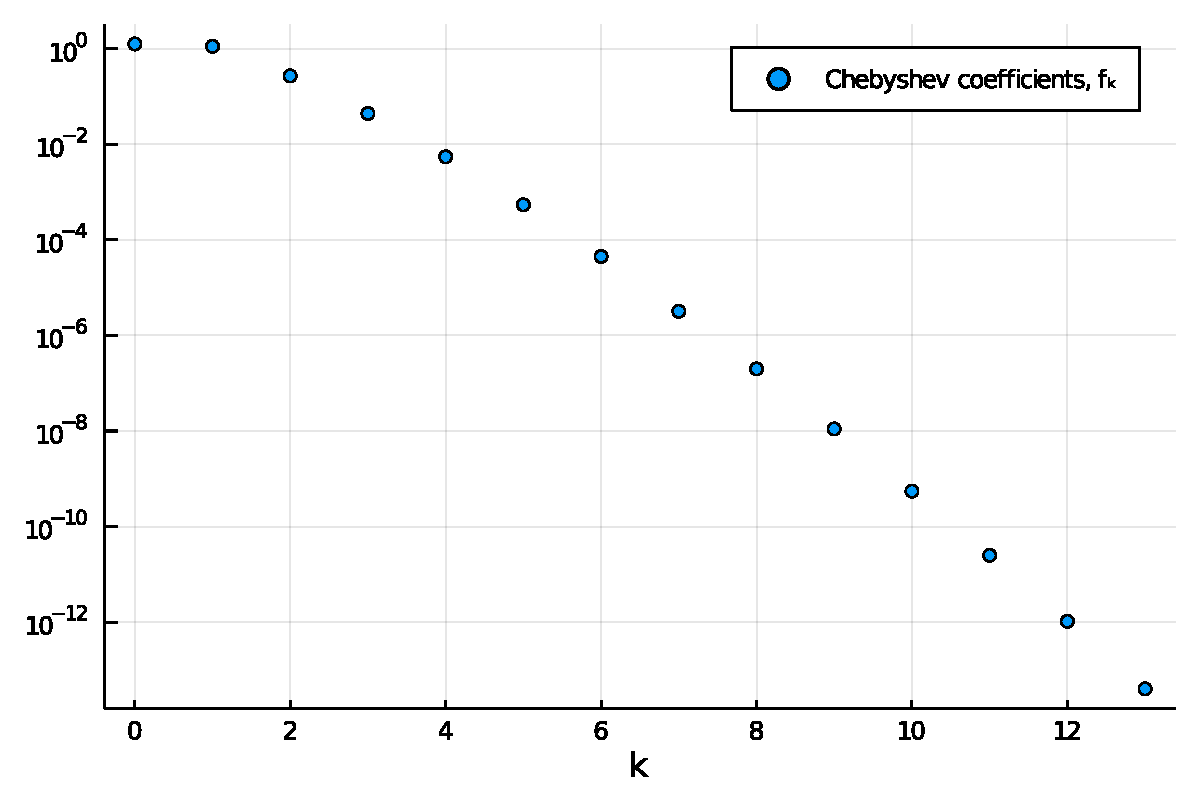
\includegraphics[width=0.7\linewidth]{C:/Users/mfaso/OneDrive/Documents/GitHub/M3M6AppliedComplexAnalysis/output/figures/Lecture19_12_1.pdf}}

\begin{lstlisting}
(*@\HLJLnd{@show}@*) (*@\HLJLnf{ncoefficients}@*)(*@\HLJLp{(}@*)(*@\HLJLn{f}@*)(*@\HLJLp{)}@*)
(*@\HLJLnd{@show}@*) (*@\HLJLnf{f}@*)(*@\HLJLp{(}@*)(*@\HLJLnfB{0.1}@*)(*@\HLJLp{)}@*) (*@\HLJLcs{{\#}}@*) (*@\HLJLcs{equivalent}@*) (*@\HLJLcs{to}@*) (*@\HLJLcs{f.coefficients{\textquotesingle}*[cos(k*acos(x))}@*) (*@\HLJLcs{for}@*) (*@\HLJLcs{k=0:ncoefficients(f)-1]}@*)
(*@\HLJLnd{@show}@*) (*@\HLJLnf{exp}@*)(*@\HLJLp{(}@*)(*@\HLJLnfB{0.1}@*)(*@\HLJLp{);}@*)
\end{lstlisting}

\begin{lstlisting}
ncoefficients(f) = 14
f(0.1) = 1.1051709180756477
exp(0.1) = 1.1051709180756477
\end{lstlisting}


The accuracy of this approximation is typically dictated by the smoothness of $f$: the more times we can differentiate, the faster it converges. For analytic functions, it's dictated by the domain of analyticity, just like Laurent/Fourier series. In the case above, $\E^x$ is entire hence we get faster than exponential convergence.

Chebyshev expansions work even when Taylor series do not. For example, the following function has poles at $\pm {\I \over 5}$, which means the radius of convergence for the Taylor series is $|x| < {1 \over 5}$, but Chebyshev polynomials continue to work on $[-1,1]$:


\begin{lstlisting}
(*@\HLJLn{f}@*) (*@\HLJLoB{=}@*) (*@\HLJLnf{Fun}@*)(*@\HLJLp{(}@*) (*@\HLJLn{x}@*) (*@\HLJLoB{->}@*) (*@\HLJLni{1}@*)(*@\HLJLoB{/}@*)(*@\HLJLp{(}@*)(*@\HLJLni{25}@*)(*@\HLJLn{x}@*)(*@\HLJLoB{{\textasciicircum}}@*)(*@\HLJLni{2}@*) (*@\HLJLoB{+}@*) (*@\HLJLni{1}@*)(*@\HLJLp{),}@*) (*@\HLJLnf{Chebyshev}@*)(*@\HLJLp{())}@*)
(*@\HLJLnd{@show}@*) (*@\HLJLnf{ncoefficients}@*)(*@\HLJLp{(}@*)(*@\HLJLn{f}@*)(*@\HLJLp{)}@*)
(*@\HLJLnf{plot}@*)(*@\HLJLp{(}@*)(*@\HLJLn{f}@*)(*@\HLJLp{)}@*)
\end{lstlisting}
\begin{lstlisting}
ncoefficients(f) = 189
\end{lstlisting}
\cent{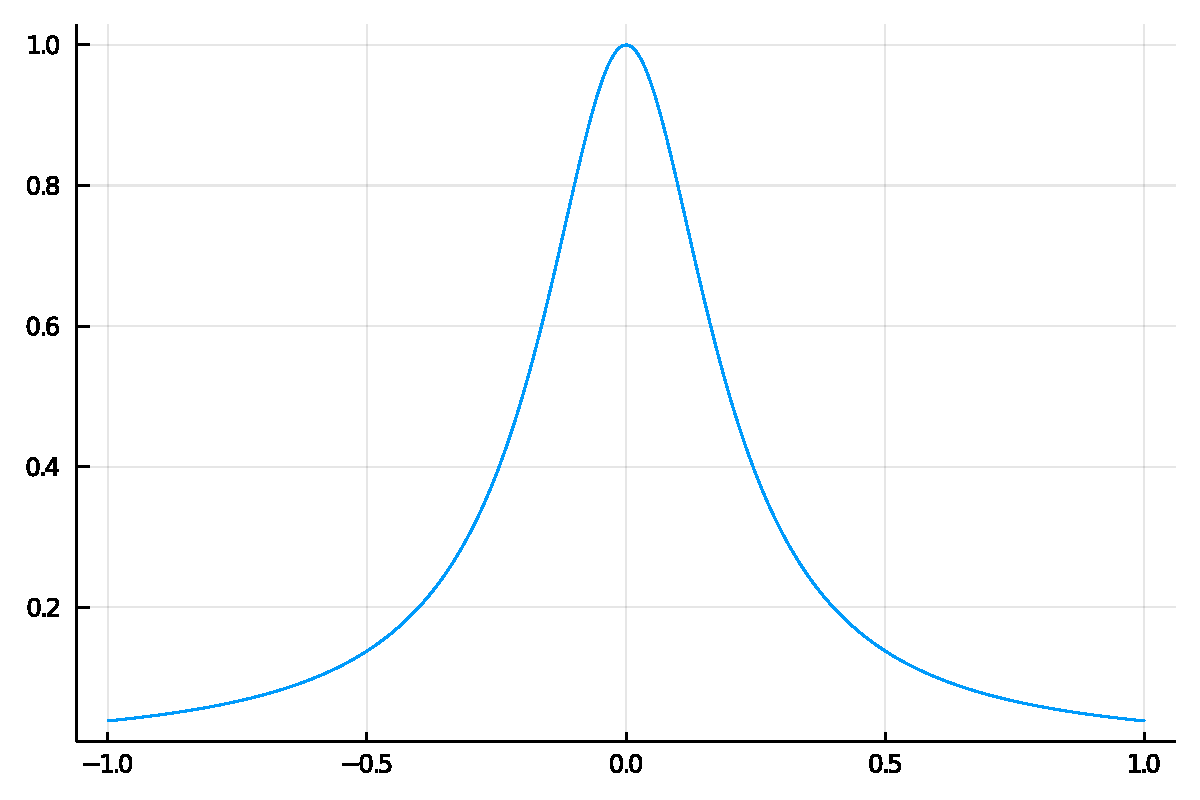
\includegraphics[width=0.5\linewidth]{C:/Users/mfaso/OneDrive/Documents/GitHub/M3M6AppliedComplexAnalysis/output/figures/Lecture19_14_1.pdf}}

This can be explained for Chebyshev expansion by noting that it is the cosine expansion / Fourier expansion of an even function:

\[
f(x) = \sum_{k=0}^\infty f_k T_k(x) \Leftrightarrow f(\cos \theta) = \sum_{k=0}^\infty f_k \cos k \theta
\]
\subsubsection{Exponential decay of Fourier coefficients of periodic, analytic functions revisited}
Before we get to the decay of Chebyshev coefficients, we revisit the proof of the exponential decay of \emph{Fourier} coefficients in Lecture 6. Suppose $f(\theta)$ is $2\pi$-periodic and analytic on $\theta \in [-\pi, \pi)$, then

\[
    f(\theta) = \sum_{k=-\infty}^\infty \hat f_k \E^{i k \theta}
\]
where

\[
\hat f_k = {1\over 2 \pi} \int_{-\pi}^\pi f(\theta) \E^{-i k \theta} d \theta.
\]
Recall in Lecture 6 we set $z = \E^{\I \theta}$ in which case the Fourier series of $f$ becomes a Laurent series of a function $g(z)$:

\[
f(\theta) = \sum_{k=-\infty}^\infty \hat f_k \E^{i k \theta} = \sum_{k=-\infty}^\infty g_k z^k =: g(z),
\]
with $g_k = \hat f_k$. We proved that if $g(z)$ is analytic on the closed annulus $A_{r,R} = \lbrace z : r \leq \vert z \vert \leq R \rbrace$, $0 < r <1$, $R > 1$ then for all $k \in \mathbb{Z}$, $|g_k | \leq M\min\left\{{1 \over R^k} , {1 \over r^k}\right\}$ where $M = \sup_{z \in  A_{r,R}} |g(z)|$. This result implies the exponential decay of the Fourier coefficients of $f$.

An annulus in the $z$-plane corresponds to a strip of width $2\pi$ in the (complex) $\theta$-plane under the transformation $z = \E^{\I \theta}$, $\Re \theta \in [-\pi, \pi)$:
\begin{align*}
& z \in A_{r,R} = \lbrace z : r \leq \vert z \vert \leq R \rbrace \qquad \underbrace{\Longleftrightarrow}_{z = \E^{\I \theta}} \\
& \theta \in  S_{r,R} =   \lbrace \theta : -\pi \leq \Re  \theta < \pi,  -\log(R) \leq \Im \theta \leq \log(1/r) \rbrace.
\end{align*}
\newpage
Suppose $f(\theta)$ is real-valued on $[-\pi, \pi)$, then $\overline{f(\theta)} = f(\overline{\theta})$. Hence if the closest singularity to the real $\theta$-axis is at $\theta = \theta_x + \I \theta_y$, with $\theta_x \in [-\pi, \pi)$ and $\theta_y > 0$, then $f$ also has a singularity at  $\theta_x - \I \theta_y$. Thus $f$ is analytic in the strip
\[
S_{r,R} = \theta \in    \lbrace \theta : -\pi \leq \Re  \theta < \pi,  -\log(R) \leq \Im \theta \leq \log(1/r) \rbrace
\]
with
\[
{1 \over r} = R < \E^{\theta_y}
\]
and the Fourier coefficients are bounded by
\[
|f_k | = |g_k |  \leq M\min\left\{{1 \over R^k} , {1 \over r^k}\right\} = M r^{|k|} = M R^{-|k|}, \qquad k \in \mathbb{Z},
\]
where $M = \sup_{z \in  A_{r,R}} |g(z)| = \sup_{\theta \in  S_{r,R}} |f(\theta)|$. The larger the strip of analyticity, the larger we can make $R$ and the faster the Fourier coefficients of $f$ decay as $\vert k \vert \to \infty$  (hence the faster the truncated Fourier expansion $\sum_{k=-n}^{n}\hat f_k \E^{i k \theta}$ of $f$ converges to $f$ as $n \to \infty$).
\newpage
\emph{Example (see also Lecture 6)} The function

\[
 f(\theta) = {1 \over 2 - \cos\theta},
\]
has poles at $\theta = \pm \I \log (2 + \sqrt{3})$; it is analytic in the strip $S_{r,R}$ with $R = 1/r < 2 + \sqrt{3}$ and the maximum of $\vert f(\theta) \vert$ on $S_{r,R}$ is

\[
M = {2 \over 4 - R^{-1} + R},
\]
hence

\[
|f_k| =     |g_k| \leq {2 \over 4 - R -R^{-1}} R^{-\vert k \vert}, \qquad k \in \mathbb{Z},
\]
for all $R < 2 + \sqrt{3}$.


\begin{lstlisting}
(*@\HLJLn{g}@*) (*@\HLJLoB{=}@*)(*@\HLJLnf{Fun}@*)(*@\HLJLp{(}@*)(*@\HLJLn{\ensuremath{\theta}}@*) (*@\HLJLoB{->}@*) (*@\HLJLni{1}@*)(*@\HLJLoB{/}@*)(*@\HLJLp{(}@*)(*@\HLJLni{2}@*)(*@\HLJLoB{-}@*)(*@\HLJLnf{cos}@*)(*@\HLJLp{(}@*)(*@\HLJLn{\ensuremath{\theta}}@*)(*@\HLJLp{)),}@*) (*@\HLJLnf{Laurent}@*)(*@\HLJLp{(}@*)(*@\HLJLoB{-}@*)(*@\HLJLn{\ensuremath{\pi}}@*) (*@\HLJLoB{..}@*) (*@\HLJLn{\ensuremath{\pi}}@*)(*@\HLJLp{))}@*)
(*@\HLJLn{g\ensuremath{\_+}}@*) (*@\HLJLoB{=}@*) (*@\HLJLn{g}@*)(*@\HLJLoB{.}@*)(*@\HLJLn{coefficients}@*)(*@\HLJLp{[}@*)(*@\HLJLni{1}@*)(*@\HLJLoB{:}@*)(*@\HLJLni{2}@*)(*@\HLJLoB{:}@*)(*@\HLJLk{end}@*)(*@\HLJLp{]}@*)
(*@\HLJLnf{scatter}@*)(*@\HLJLp{(}@*)(*@\HLJLn{abs}@*)(*@\HLJLoB{.}@*)(*@\HLJLp{(}@*)(*@\HLJLn{g\ensuremath{\_+}}@*)(*@\HLJLp{);}@*) (*@\HLJLn{yscale}@*)(*@\HLJLoB{=:}@*)(*@\HLJLn{log10}@*)(*@\HLJLp{,}@*) (*@\HLJLn{label}@*)(*@\HLJLoB{=}@*)(*@\HLJLs{"{}|g{\_}k|"{}}@*)(*@\HLJLp{,}@*) (*@\HLJLn{legend}@*)(*@\HLJLoB{=:}@*)(*@\HLJLn{bottomleft}@*)(*@\HLJLp{,}@*)(*@\HLJLn{xlabel}@*)(*@\HLJLoB{=}@*)(*@\HLJLs{"{}k"{}}@*)(*@\HLJLp{)}@*)
(*@\HLJLn{R}@*) (*@\HLJLoB{=}@*) (*@\HLJLnfB{1.1}@*)
(*@\HLJLnf{scatter!}@*)(*@\HLJLp{(}@*)(*@\HLJLni{2}@*)(*@\HLJLoB{/}@*)(*@\HLJLp{(}@*)(*@\HLJLni{4}@*)(*@\HLJLoB{-}@*)(*@\HLJLn{R}@*)(*@\HLJLoB{-}@*)(*@\HLJLnf{inv}@*)(*@\HLJLp{(}@*)(*@\HLJLn{R}@*)(*@\HLJLp{))}@*)(*@\HLJLoB{*}@*)(*@\HLJLn{R}@*)(*@\HLJLoB{.{\textasciicircum}}@*)(*@\HLJLp{(}@*)(*@\HLJLoB{-}@*)(*@\HLJLp{(}@*)(*@\HLJLni{0}@*)(*@\HLJLoB{:}@*)(*@\HLJLnf{length}@*)(*@\HLJLp{(}@*)(*@\HLJLn{g\ensuremath{\_+}}@*)(*@\HLJLp{))),}@*) (*@\HLJLn{label}@*) (*@\HLJLoB{=}@*) (*@\HLJLs{"{}R}@*) (*@\HLJLs{=}@*) (*@\HLJLsi{{\$}R}@*)(*@\HLJLs{"{}}@*)(*@\HLJLp{)}@*)
(*@\HLJLn{R}@*) (*@\HLJLoB{=}@*) (*@\HLJLnfB{3.5}@*)
(*@\HLJLnf{scatter!}@*)(*@\HLJLp{(}@*)(*@\HLJLni{2}@*)(*@\HLJLoB{/}@*)(*@\HLJLp{(}@*)(*@\HLJLni{4}@*)(*@\HLJLoB{-}@*)(*@\HLJLn{R}@*)(*@\HLJLoB{-}@*)(*@\HLJLnf{inv}@*)(*@\HLJLp{(}@*)(*@\HLJLn{R}@*)(*@\HLJLp{))}@*)(*@\HLJLoB{*}@*)(*@\HLJLn{R}@*)(*@\HLJLoB{.{\textasciicircum}}@*)(*@\HLJLp{(}@*)(*@\HLJLoB{-}@*)(*@\HLJLp{(}@*)(*@\HLJLni{0}@*)(*@\HLJLoB{:}@*)(*@\HLJLnf{length}@*)(*@\HLJLp{(}@*)(*@\HLJLn{g\ensuremath{\_+}}@*)(*@\HLJLp{))),}@*) (*@\HLJLn{label}@*) (*@\HLJLoB{=}@*) (*@\HLJLs{"{}R}@*) (*@\HLJLs{=}@*) (*@\HLJLsi{{\$}R}@*)(*@\HLJLs{"{}}@*)(*@\HLJLp{)}@*)
(*@\HLJLn{R}@*) (*@\HLJLoB{=}@*) (*@\HLJLni{2}@*)(*@\HLJLoB{+}@*)(*@\HLJLnf{sqrt}@*)(*@\HLJLp{(}@*)(*@\HLJLni{3}@*)(*@\HLJLp{)}@*)(*@\HLJLoB{-}@*)(*@\HLJLnfB{0.1}@*)
(*@\HLJLnf{scatter!}@*)(*@\HLJLp{(}@*)(*@\HLJLni{2}@*)(*@\HLJLoB{/}@*)(*@\HLJLp{(}@*)(*@\HLJLni{4}@*)(*@\HLJLoB{-}@*)(*@\HLJLn{R}@*)(*@\HLJLoB{-}@*)(*@\HLJLnf{inv}@*)(*@\HLJLp{(}@*)(*@\HLJLn{R}@*)(*@\HLJLp{))}@*)(*@\HLJLoB{*}@*)(*@\HLJLn{R}@*)(*@\HLJLoB{.{\textasciicircum}}@*)(*@\HLJLp{(}@*)(*@\HLJLoB{-}@*)(*@\HLJLp{(}@*)(*@\HLJLni{0}@*)(*@\HLJLoB{:}@*)(*@\HLJLnf{length}@*)(*@\HLJLp{(}@*)(*@\HLJLn{g\ensuremath{\_+}}@*)(*@\HLJLp{))),}@*) (*@\HLJLn{label}@*) (*@\HLJLoB{=}@*) (*@\HLJLs{"{}R}@*) (*@\HLJLs{=}@*) (*@\HLJLsi{{\$}R}@*)(*@\HLJLs{"{}}@*)(*@\HLJLp{)}@*)
\end{lstlisting}

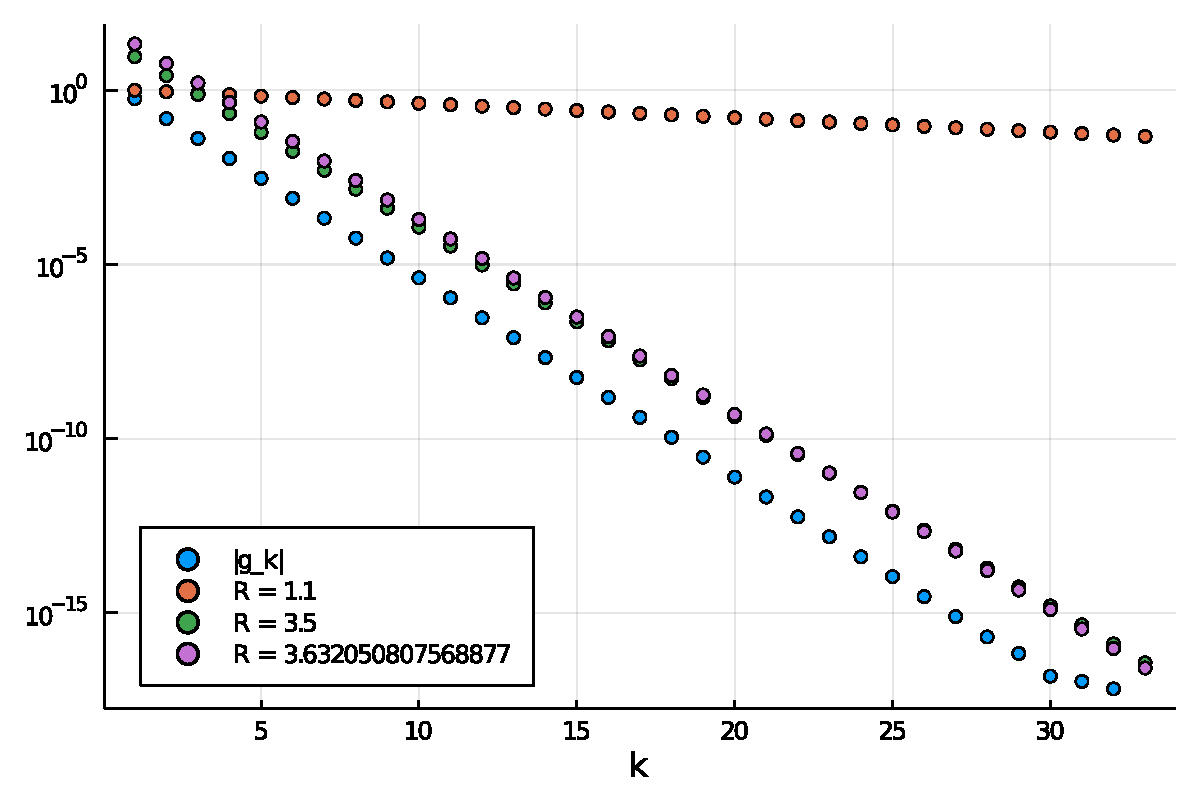
\includegraphics[width=\linewidth]{C:/Users/mfaso/OneDrive/Documents/GitHub/M3M6AppliedComplexAnalysis/output/figures/Lecture19_15_1.pdf}

\subsubsection{Exponential decay of Chebyshev coefficients of analytic functions}
Suppose $f(x)$ is analytic on $[-1, 1]$, then
\begin{align*}
f(x) & = \sum_{k = 0}^{\infty} f_k T_k(x) \\
     & =\sum_{k = 0}^{\infty} f_k \cos k\theta \qquad (x = \cos\theta) \\
     & = \sum_{k = 0}^{\infty} {f_k \over 2}\left( z^k + z^{-k}\right)  \qquad (z = \E^{\I \theta}) \\
     & =: \sum_{k = -\infty}^{\infty} g_k z^{k} =: g(z) \qquad (g_0 = f_0, g_{k} = g_{-k} = f_k/2, k\geq 0)
\end{align*}
Now we can use the bound on the Laurent coefficients of $g(z)$ to bound the Chebyshev coefficients of $f(x)$. First we need to establish what is the image in the (complex) $x$-plane of an annulus in the $z$-plane under the transformation $2x = z + z^{-1}$, which is known as the Joukowsky map.
\newpage

Let $\rho > 1$ and
\[
A_{1,\rho} =  \lbrace z : 1 \leq \vert z \vert \leq \rho \rbrace, \qquad  A_{\rho^{-1},1} =  \lbrace z : \rho^{-1} \leq \vert z \vert \leq 1 \rbrace.
\]
The Joukowsky transformation maps $A_{1,\rho}$ and $A_{\rho^{-1},1}$ to the following ellipse (known as a Bernstein ellipse) in the $x$-plane:
\[
E_{\rho} = \left\lbrace x : {(\Re x)^2 \over \alpha^2} + {(\Im x)^2 \over \beta^2} \leq 1, \alpha = {1 \over 2}\left( \rho + \rho^{-1} \right),   \beta = {1 \over 2}\left( \rho - \rho^{-1} \right) \right\rbrace.
\]
\newpage
We conclude that if $f(x)$ is analytic on $E_{\rho}$ (or $g(z)$ is analytic on $A_{\rho^{-1},\rho}$) and $M = \sup_{x \in  E_{\rho}} |f(x)| = \sup_{z \in  A_{\rho^{-1},\rho}} |g(z)|$, then
\[
\vert f_k \vert = 2 \vert g_k \vert \leq 2M\rho^{-k}, \qquad k \geq 1.
\]
The larger the Bernstein ellipse on which $f(x)$ is analytic, the faster the decay of the Chebyshev coefficients as $k \to \infty$ (and hence the faster the convergence of the Chebyshev expansion of $f$).
A truncated Chebyshev expansion with $n$ terms of a function $f(x)$ that is analytic on $E_{\rho}$ converges at essentially the same exponential rate as the bound on the Chebyshev coefficients as $n \to \infty$:
\[
\left \vert f(x) -   \sum_{k = 0}^{n-1}f_kT_k(x) \right\vert  = \left \vert  \sum_{k = n}^{\infty}f_kT_k(x) \right\vert \leq \sum_{k = n}^{\infty}\vert f_k \vert \leq 2M \sum_{k = n}^{\infty} \rho^{-k} = 2M \frac{\rho^{-n}}{1 - \rho^{-1}}
\]

\newpage
\emph{Example}  In the case of $f(x) = {1 \over 25 x^2 + 1}$, setting $2x = z + z^{-1}$, we find that

\[
f(x) = f\left( {z+z^{-1} \over 2 } \right) = g(z) = {4 z^2 \over 25 + 54 z^2 + 25 z^4}.
\]
In the complex $x$-plane, $f(x)$ has poles at $\pm \I/5$ and is analytic on $E_{\rho}$ with $\beta = (\rho - \rho^{-1})/2 < 1/5$, hence $\rho < { 1 + \sqrt{26} \over 5 }$. In the $z$-plane, $g(z)$ has poles at $\pm \I { 1 \pm \sqrt{26} \over 5 } \approx \pm 0.8198040\I,\pm1.2198\I$ and is analytic on the annulus $\rho^{-1} \leq \vert z \vert \leq \rho$.


\begin{lstlisting}
(*@\HLJLn{\ensuremath{\rho}}@*) (*@\HLJLoB{=}@*) (*@\HLJLp{(}@*)(*@\HLJLni{1}@*) (*@\HLJLoB{+}@*) (*@\HLJLnf{sqrt}@*)(*@\HLJLp{(}@*)(*@\HLJLni{26}@*)(*@\HLJLp{))}@*)(*@\HLJLoB{/}@*)(*@\HLJLni{5}@*)(*@\HLJLoB{-}@*)(*@\HLJLnfB{0.05}@*)(*@\HLJLp{;}@*)
(*@\HLJLn{\ensuremath{\alpha}}@*) (*@\HLJLoB{=}@*) (*@\HLJLp{(}@*)(*@\HLJLn{\ensuremath{\rho}}@*) (*@\HLJLoB{+}@*) (*@\HLJLni{1}@*)(*@\HLJLoB{/}@*)(*@\HLJLn{\ensuremath{\rho}}@*)(*@\HLJLp{)}@*)(*@\HLJLoB{/}@*)(*@\HLJLni{2}@*)
(*@\HLJLn{\ensuremath{\beta}}@*) (*@\HLJLoB{=}@*) (*@\HLJLp{(}@*)(*@\HLJLn{\ensuremath{\rho}}@*) (*@\HLJLoB{-}@*) (*@\HLJLni{1}@*)(*@\HLJLoB{/}@*)(*@\HLJLn{\ensuremath{\rho}}@*)(*@\HLJLp{)}@*)(*@\HLJLoB{/}@*)(*@\HLJLni{2}@*)
(*@\HLJLn{\ensuremath{\theta}}@*) (*@\HLJLoB{=}@*) (*@\HLJLoB{-}@*)(*@\HLJLn{\ensuremath{\pi}}@*)(*@\HLJLoB{:}@*)(*@\HLJLnfB{0.01}@*)(*@\HLJLoB{:}@*)(*@\HLJLn{\ensuremath{\pi}}@*)
(*@\HLJLn{f}@*) (*@\HLJLoB{=}@*) (*@\HLJLn{x}@*) (*@\HLJLoB{->}@*) (*@\HLJLni{1}@*)(*@\HLJLoB{/}@*)(*@\HLJLp{(}@*)(*@\HLJLni{25}@*)(*@\HLJLn{x}@*)(*@\HLJLoB{{\textasciicircum}}@*)(*@\HLJLni{2}@*) (*@\HLJLoB{+}@*) (*@\HLJLni{1}@*)(*@\HLJLp{)}@*)
(*@\HLJLnf{phaseplot}@*)(*@\HLJLp{(}@*)(*@\HLJLoB{-}@*)(*@\HLJLnfB{2..2}@*)(*@\HLJLp{,}@*) (*@\HLJLoB{-}@*)(*@\HLJLnfB{2..2}@*)(*@\HLJLp{,}@*) (*@\HLJLn{z}@*) (*@\HLJLoB{->}@*) (*@\HLJLnf{f}@*)(*@\HLJLp{(}@*)(*@\HLJLn{z}@*)(*@\HLJLp{))}@*)
(*@\HLJLnf{plot!}@*)(*@\HLJLp{(}@*)(*@\HLJLn{\ensuremath{\alpha}}@*)(*@\HLJLoB{*}@*)(*@\HLJLn{cos}@*)(*@\HLJLoB{.}@*)(*@\HLJLp{(}@*)(*@\HLJLn{\ensuremath{\theta}}@*)(*@\HLJLp{),}@*)(*@\HLJLn{\ensuremath{\beta}}@*)(*@\HLJLoB{*}@*)(*@\HLJLn{sin}@*)(*@\HLJLoB{.}@*)(*@\HLJLp{(}@*)(*@\HLJLn{\ensuremath{\theta}}@*)(*@\HLJLp{);}@*)(*@\HLJLn{linecolor}@*)(*@\HLJLoB{=}@*)(*@\HLJLs{"{}black"{}}@*)(*@\HLJLp{,}@*)(*@\HLJLn{label}@*)(*@\HLJLoB{=}@*)(*@\HLJLs{"{}Bernstein}@*) (*@\HLJLs{ellipse"{}}@*)(*@\HLJLp{)}@*)
\end{lstlisting}

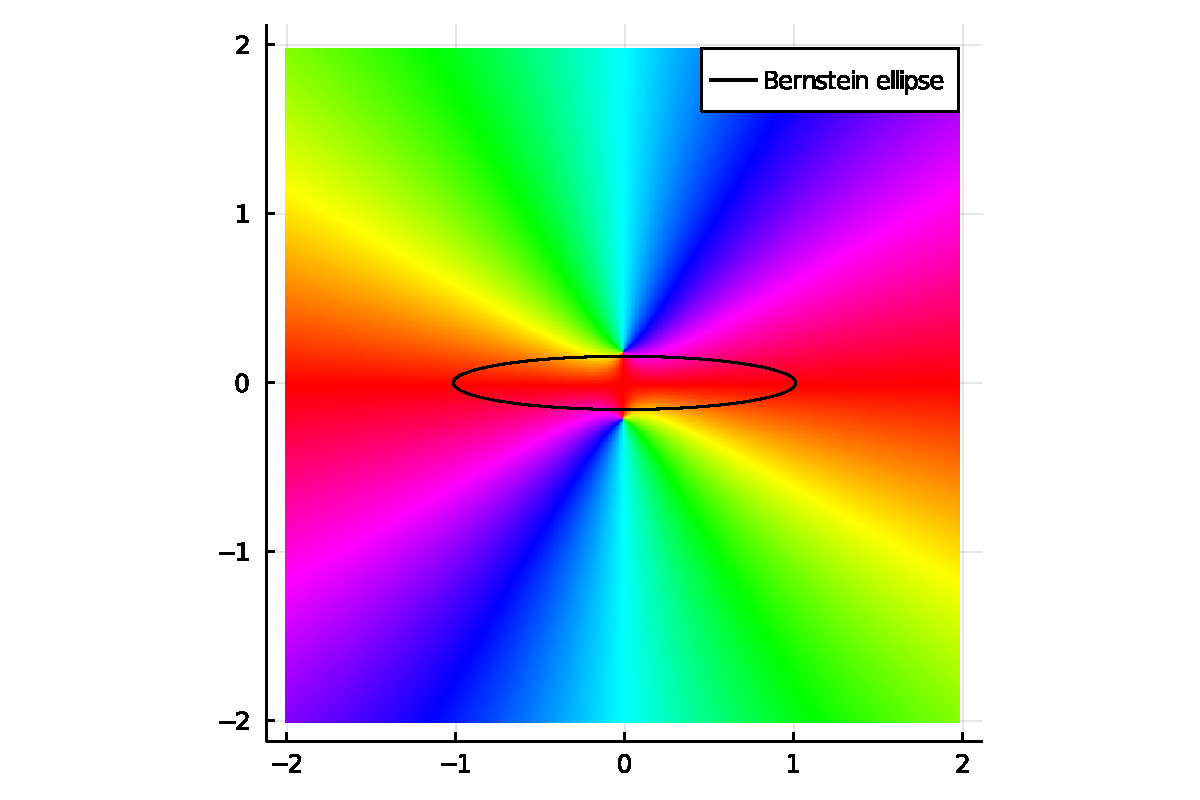
\includegraphics[width=\linewidth]{C:/Users/mfaso/OneDrive/Documents/GitHub/M3M6AppliedComplexAnalysis/output/figures/Lecture19_16_1.pdf}
\newpage
\begin{lstlisting}
(*@\HLJLnf{phaseplot}@*)(*@\HLJLp{(}@*)(*@\HLJLoB{-}@*)(*@\HLJLnfB{3..3}@*)(*@\HLJLp{,}@*) (*@\HLJLoB{-}@*)(*@\HLJLnfB{3..3}@*)(*@\HLJLp{,}@*) (*@\HLJLn{z}@*) (*@\HLJLoB{->}@*) (*@\HLJLnf{f}@*)(*@\HLJLp{((}@*)(*@\HLJLn{z}@*)(*@\HLJLoB{+}@*)(*@\HLJLni{1}@*)(*@\HLJLoB{/}@*)(*@\HLJLn{z}@*)(*@\HLJLp{)}@*)(*@\HLJLoB{/}@*)(*@\HLJLni{2}@*)(*@\HLJLp{))}@*)
(*@\HLJLnf{plot!}@*)(*@\HLJLp{(}@*)(*@\HLJLn{\ensuremath{\rho}}@*)(*@\HLJLoB{*}@*)(*@\HLJLn{cos}@*)(*@\HLJLoB{.}@*)(*@\HLJLp{(}@*)(*@\HLJLn{\ensuremath{\theta}}@*)(*@\HLJLp{),}@*)(*@\HLJLn{\ensuremath{\rho}}@*)(*@\HLJLoB{*}@*)(*@\HLJLn{sin}@*)(*@\HLJLoB{.}@*)(*@\HLJLp{(}@*)(*@\HLJLn{\ensuremath{\theta}}@*)(*@\HLJLp{),}@*)(*@\HLJLn{linecolor}@*)(*@\HLJLoB{=}@*)(*@\HLJLs{"{}black"{}}@*)(*@\HLJLp{,}@*)(*@\HLJLn{label}@*)(*@\HLJLoB{=}@*)(*@\HLJLs{"{}|z|}@*) (*@\HLJLs{=}@*) (*@\HLJLs{\ensuremath{\rho}"{}}@*)(*@\HLJLp{)}@*)
(*@\HLJLnf{plot!}@*)(*@\HLJLp{(}@*)(*@\HLJLn{cos}@*)(*@\HLJLoB{.}@*)(*@\HLJLp{(}@*)(*@\HLJLn{\ensuremath{\theta}}@*)(*@\HLJLp{)}@*)(*@\HLJLoB{/}@*)(*@\HLJLn{\ensuremath{\rho}}@*)(*@\HLJLp{,}@*)(*@\HLJLn{sin}@*)(*@\HLJLoB{.}@*)(*@\HLJLp{(}@*)(*@\HLJLn{\ensuremath{\theta}}@*)(*@\HLJLp{)}@*)(*@\HLJLoB{/}@*)(*@\HLJLn{\ensuremath{\rho}}@*)(*@\HLJLp{,}@*)(*@\HLJLn{linecolor}@*)(*@\HLJLoB{=}@*)(*@\HLJLs{"{}black"{}}@*)(*@\HLJLp{,}@*)(*@\HLJLn{label}@*)(*@\HLJLoB{=}@*)(*@\HLJLs{"{}|z|}@*) (*@\HLJLs{=}@*) (*@\HLJLs{1/\ensuremath{\rho}"{}}@*)(*@\HLJLp{)}@*)
\end{lstlisting}

\cent{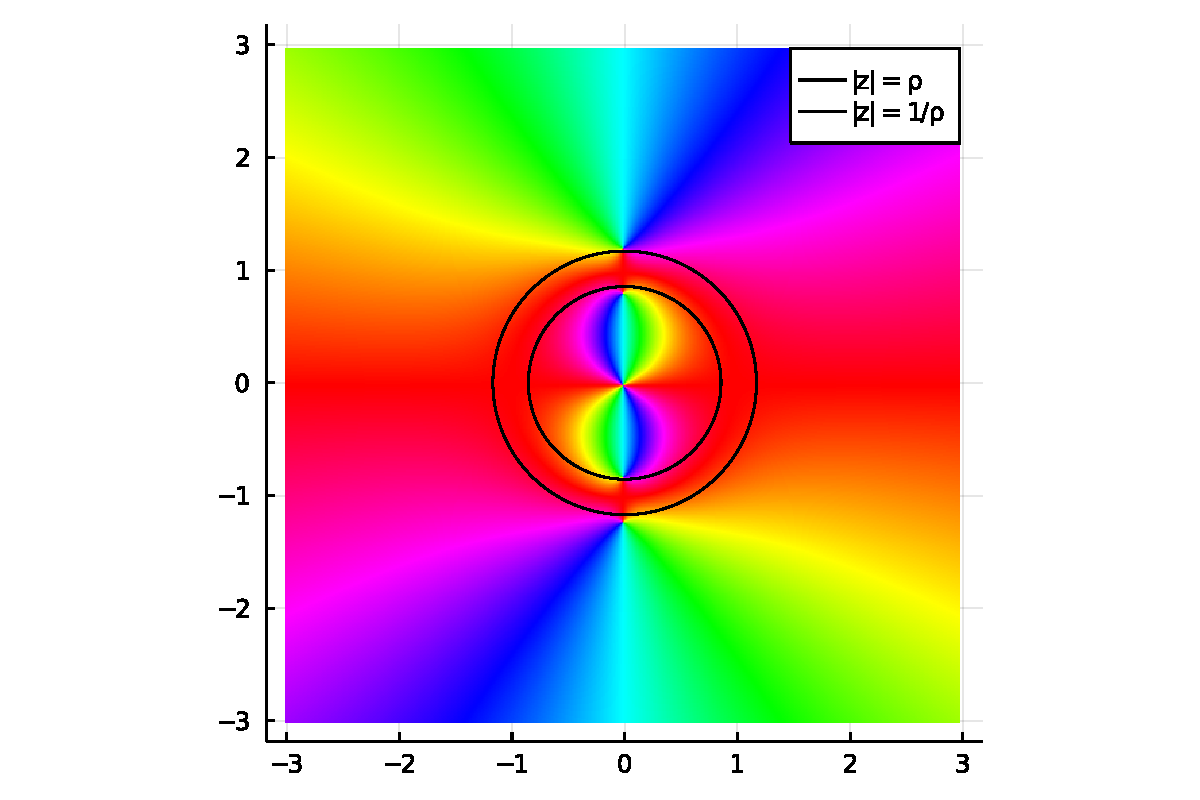
\includegraphics[width=0.925\linewidth]{C:/Users/mfaso/OneDrive/Documents/GitHub/M3M6AppliedComplexAnalysis/output/figures/Lecture19_17_1.pdf}}

For $\beta = (\rho - \rho^{-1})/2 < 1/5$, we have

\[
M =  \sup_{x \in  E_{\rho}} |f(x)| = {1 \over 1 - 25 \beta^2}
\]
hence for $k \geq 1$,

\[
\vert f_k \vert \leq {2 \over   1 - 25 \beta^2} \rho^{-k}, \qquad 1 < \rho <  { 1 + \sqrt{26} \over 5 }.
\]
Therefore we predict a rate of decay of about $1.2198^{-k}$:


\begin{lstlisting}
(*@\HLJLnf{bound}@*)(*@\HLJLp{(}@*)(*@\HLJLn{\ensuremath{\beta}}@*)(*@\HLJLp{,}@*)(*@\HLJLn{k}@*)(*@\HLJLp{)}@*) (*@\HLJLoB{=}@*) (*@\HLJLni{2}@*)(*@\HLJLoB{/}@*)(*@\HLJLp{(}@*)(*@\HLJLni{1}@*)(*@\HLJLoB{-}@*)(*@\HLJLni{25}@*)(*@\HLJLoB{*}@*)(*@\HLJLn{\ensuremath{\beta}}@*)(*@\HLJLoB{{\textasciicircum}}@*)(*@\HLJLni{2}@*)(*@\HLJLp{)}@*)(*@\HLJLoB{*}@*)(*@\HLJLp{(}@*)(*@\HLJLn{\ensuremath{\beta}}@*) (*@\HLJLoB{+}@*) (*@\HLJLnf{sqrt}@*)(*@\HLJLp{(}@*)(*@\HLJLn{\ensuremath{\beta}}@*)(*@\HLJLoB{{\textasciicircum}}@*)(*@\HLJLni{2}@*) (*@\HLJLoB{+}@*) (*@\HLJLni{1}@*)(*@\HLJLp{))}@*)(*@\HLJLoB{{\textasciicircum}}@*)(*@\HLJLp{(}@*)(*@\HLJLoB{-}@*)(*@\HLJLn{k}@*)(*@\HLJLp{)}@*)
(*@\HLJLn{f}@*) (*@\HLJLoB{=}@*) (*@\HLJLnf{Fun}@*)(*@\HLJLp{(}@*) (*@\HLJLn{x}@*) (*@\HLJLoB{->}@*) (*@\HLJLni{1}@*)(*@\HLJLoB{/}@*)(*@\HLJLp{(}@*)(*@\HLJLni{25}@*)(*@\HLJLn{x}@*)(*@\HLJLoB{{\textasciicircum}}@*)(*@\HLJLni{2}@*) (*@\HLJLoB{+}@*) (*@\HLJLni{1}@*)(*@\HLJLp{),}@*) (*@\HLJLnf{Chebyshev}@*)(*@\HLJLp{())}@*)
(*@\HLJLnf{scatter}@*)(*@\HLJLp{(}@*)(*@\HLJLn{abs}@*)(*@\HLJLoB{.}@*)(*@\HLJLp{(}@*)(*@\HLJLn{f}@*)(*@\HLJLoB{.}@*)(*@\HLJLn{coefficients}@*)(*@\HLJLp{)}@*) (*@\HLJLoB{.+}@*) (*@\HLJLnf{eps}@*)(*@\HLJLp{();}@*) (*@\HLJLn{yscale}@*)(*@\HLJLoB{=:}@*)(*@\HLJLn{log10}@*)(*@\HLJLp{,}@*) (*@\HLJLn{label}@*)(*@\HLJLoB{=}@*)(*@\HLJLs{"{}Chebyshev}@*) (*@\HLJLs{coefficients"{}}@*)(*@\HLJLp{)}@*)
(*@\HLJLnf{plot!}@*)(*@\HLJLp{(}@*)(*@\HLJLni{1}@*)(*@\HLJLoB{:}@*)(*@\HLJLnf{ncoefficients}@*)(*@\HLJLp{(}@*)(*@\HLJLn{f}@*)(*@\HLJLp{),}@*) (*@\HLJLn{bound}@*)(*@\HLJLoB{.}@*)(*@\HLJLp{(}@*)(*@\HLJLni{1}@*)(*@\HLJLoB{/}@*)(*@\HLJLni{5}@*)(*@\HLJLoB{-}@*)(*@\HLJLnfB{0.001}@*)(*@\HLJLp{,}@*)(*@\HLJLni{1}@*)(*@\HLJLoB{:}@*)(*@\HLJLnf{ncoefficients}@*)(*@\HLJLp{(}@*)(*@\HLJLn{f}@*)(*@\HLJLp{));}@*) (*@\HLJLn{label}@*)(*@\HLJLoB{=}@*)(*@\HLJLs{"{}upper}@*) (*@\HLJLs{bound"{}}@*)(*@\HLJLp{)}@*)
(*@\HLJLcs{{\#}}@*) (*@\HLJLcs{Also}@*) (*@\HLJLcs{calculate}@*) (*@\HLJLcs{the}@*) (*@\HLJLcs{error}@*) (*@\HLJLcs{of}@*) (*@\HLJLcs{truncated}@*) (*@\HLJLcs{Chebyshev}@*) (*@\HLJLcs{expansions}@*) (*@\HLJLcs{with}@*) (*@\HLJLcs{n}@*) (*@\HLJLcs{terms}@*) (*@\HLJLcs{for}@*) (*@\HLJLcs{n}@*) (*@\HLJLcs{=}@*) (*@\HLJLcs{1,}@*) (*@\HLJLcs{2,}@*) (*@\HLJLcs{...}@*)
(*@\HLJLn{xx}@*) (*@\HLJLoB{=}@*) (*@\HLJLoB{-}@*)(*@\HLJLni{1}@*)(*@\HLJLoB{:}@*)(*@\HLJLnfB{0.001}@*)(*@\HLJLoB{:}@*)(*@\HLJLni{1}@*) (*@\HLJLcs{{\#}}@*) (*@\HLJLcs{a}@*) (*@\HLJLcs{fine}@*) (*@\HLJLcs{grid}@*) (*@\HLJLcs{on}@*) (*@\HLJLcs{which}@*) (*@\HLJLcs{to}@*) (*@\HLJLcs{evaluate}@*)
(*@\HLJLn{Errv}@*) (*@\HLJLoB{=}@*) (*@\HLJLp{[(}@*)(*@\HLJLnf{maximum}@*)(*@\HLJLp{(}@*)(*@\HLJLn{abs}@*)(*@\HLJLoB{.}@*)(*@\HLJLp{(}@*)(*@\HLJLn{f}@*)(*@\HLJLoB{.}@*)(*@\HLJLp{(}@*)(*@\HLJLn{xx}@*)(*@\HLJLp{)}@*)(*@\HLJLoB{-}@*)(*@\HLJLnf{Fun}@*)(*@\HLJLp{(}@*)(*@\HLJLn{f}@*)(*@\HLJLp{,}@*)(*@\HLJLnf{Chebyshev}@*)(*@\HLJLp{(),}@*)(*@\HLJLn{n}@*)(*@\HLJLp{)}@*)(*@\HLJLoB{.}@*)(*@\HLJLp{(}@*)(*@\HLJLn{xx}@*)(*@\HLJLp{))))}@*) (*@\HLJLk{for}@*) (*@\HLJLn{n}@*) (*@\HLJLoB{=}@*) (*@\HLJLni{1}@*)(*@\HLJLoB{:}@*)(*@\HLJLnf{ncoefficients}@*)(*@\HLJLp{(}@*)(*@\HLJLn{f}@*)(*@\HLJLp{)]}@*)
(*@\HLJLnf{scatter!}@*)(*@\HLJLp{(}@*)(*@\HLJLni{1}@*)(*@\HLJLoB{:}@*)(*@\HLJLnf{ncoefficients}@*)(*@\HLJLp{(}@*)(*@\HLJLn{f}@*)(*@\HLJLp{),}@*)(*@\HLJLn{Errv}@*)(*@\HLJLoB{.+}@*)(*@\HLJLnf{eps}@*)(*@\HLJLp{();}@*)(*@\HLJLn{label}@*)(*@\HLJLoB{=}@*)(*@\HLJLs{"{}truncated}@*) (*@\HLJLs{expansion}@*) (*@\HLJLs{error"{}}@*)(*@\HLJLp{)}@*)
(*@\HLJLnf{plot!}@*)(*@\HLJLp{(}@*) (*@\HLJLnfB{1.2198}@*)(*@\HLJLoB{.{\textasciicircum}}@*)(*@\HLJLp{(}@*)(*@\HLJLoB{-}@*)(*@\HLJLp{(}@*)(*@\HLJLni{0}@*)(*@\HLJLoB{:}@*)(*@\HLJLnf{ncoefficients}@*)(*@\HLJLp{(}@*)(*@\HLJLn{f}@*)(*@\HLJLp{)));}@*) (*@\HLJLn{label}@*)(*@\HLJLoB{=}@*)(*@\HLJLs{"{}\ensuremath{\rho}{\textasciicircum}(-k)"{}}@*)(*@\HLJLp{)}@*)
\end{lstlisting}


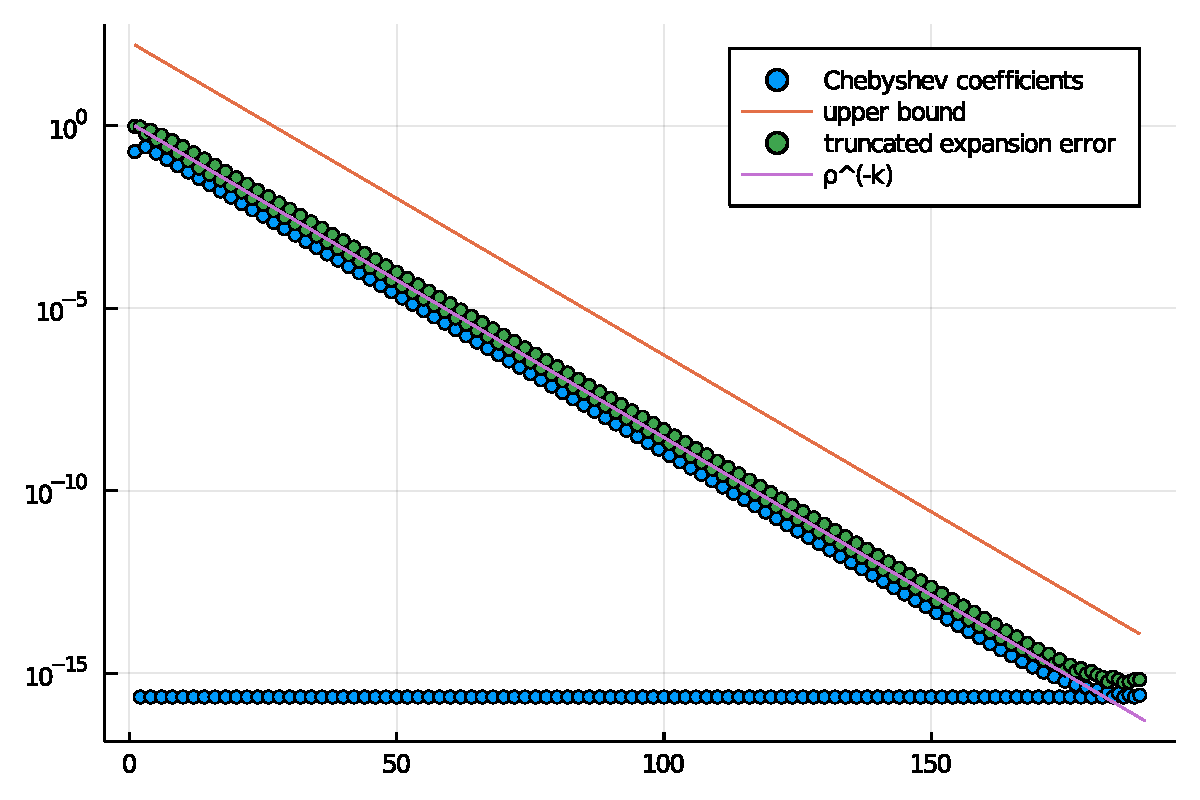
\includegraphics[width=\linewidth]{C:/Users/mfaso/OneDrive/Documents/GitHub/M3M6AppliedComplexAnalysis/output/figures/Lecture19_18_1.pdf}

}
\end{document}
